\documentclass[danish ,a4paper,12pt]{article}
\usepackage[utf8]{inputenc}
\usepackage[table]{xcolor}% http://ctan.org/pkg/xcolor
\title{Bachelor projekt}
\author{msan18 }
\date{Juni 2021}

\usepackage{booktabs}
\usepackage{multirow}
\usepackage{rotating}
\usepackage{soul}
\usepackage[utf8]{inputenc}
%\usepackage[english]{babel}
\usepackage{apacite}
\usepackage[square,numbers]{natbib}
\bibliographystyle{apacite}
\usepackage{import}


%Title and author
\title{Bibliography management: \texttt{natbib} package}
\author{overleaf}
\date{}
\usepackage{amsmath}
\usepackage{wrapfig}
\usepackage{amsfonts}
\usepackage{amssymb}
\usepackage{graphicx}
\setcitestyle{authoryear,open={(},close={)}}
\graphicspath{ {./images/} }
\usepackage{url}
\usepackage{csquotes}
\usepackage{fullpage}
\usepackage{tabularx}
\usepackage{dcolumn}
\usepackage{float}
\usepackage{caption}
\usepackage{makecell}
\renewcommand\theadfont{\bfseries}
\usepackage{threeparttable}
\usepackage[colorlinks=true, hypertexnames=true, linkcolor=black, citecolor=black, urlcolor=black]{hyperref}
\usepackage{pdflscape}
\usepackage{rotating}
\usepackage{dcolumn}
\usepackage{blkarray}
\usepackage{array}
\usepackage{eurosym}
\usepackage{longtable}
\usepackage[]{multirow}
\usepackage{csquotes}
\usepackage{epstopdf}
\usepackage{soul}
\usepackage{float}
\usepackage{rotfloat}
\usepackage{subcaption}
\usepackage{parskip}
\usepackage{enumitem}
\usepackage{placeins}
\usepackage{tikz}
\usepackage{listings}
\usepackage{setspace}
\usepackage[bottom]{footmisc}



\usepackage[a4paper,margin=1in,headheight=.4in,headsep=12pt,heightrounded]{geometry}
\usepackage{fancyhdr}
\usetikzlibrary{arrows,automata,positioning, fit, calc}
\tikzset{
    state/.style={
           rectangle,
           rounded corners,
           draw=black, very thick,
           minimum height=2em,
           inner sep=4pt,
           text centered,
           },
}

\usepackage[T1]{fontenc}
%\usepackage[table,xcdraw]{xcolor}
\renewcommand{\figurename}{\textbf{Figure}}
\renewcommand{\tablename}{Table}

%\addto\captionsenglish{\renewcommand{\appendixname}{Appendiks}}
%\usepackage[title]{appendix}





\setlength\parindent{15pt}
\newcommand{\dd}[1]{\mathrm{d}#1}

\makeatletter
% make numeric styles use name format
\patchcmd{\NAT@test}{\else \NAT@nm}{\else \NAT@nmfmt{\NAT@nm}}{}{}
% define \citepos just like \citet
\DeclareRobustCommand\citepos
  {\begingroup
   \let\NAT@nmfmt\NAT@posfmt% ...except with a different name format
   \NAT@swafalse\let\NAT@ctype\z@\NAT@partrue
   \@ifstar{\NAT@fulltrue\NAT@citetp}{\NAT@fullfalse\NAT@citetp}}
\let\NAT@orig@nmfmt\NAT@nmfmt
\def\NAT@posfmt#1{\NAT@orig@nmfmt{#1's}}
\makeatother
\raggedbottom
\usepackage{ragged2e}
\definecolor{numbercolor}{gray}{0.7}		% Definerer en farve til brug til kapiteludseende



\pagestyle{headings}


\pagestyle{fancy}
\fancyhf{}
\rhead{Københavns Universitet}
\fancyhead[LE]{\nouppercase{\rightmark}}
\rfoot{Page \thepage}

\patchcmd{\maketitle}{\@fnsymbol}{\@arabic}{}{}
% \patchcmd{\maketitle}{\setcounter{footnote}{0}}{}{}{}
\makeatother

\makeatletter
\pgfdeclaregenericanchor{top base}{%
  \csname pgf@anchor@#1@north\endcsname
  \pgf@anchor@generic@top@base@main
}
\pgfdeclaregenericanchor{top base west}{%
  \csname pgf@anchor@#1@north west\endcsname
  \pgf@anchor@generic@top@base@main
}
\pgfdeclaregenericanchor{top base east}{%
  \csname pgf@anchor@#1@north east\endcsname
  \pgf@anchor@generic@top@base@main
}
\def\pgf@anchor@generic@top@base@main{%
  {%
    \pgfmathsetlength\pgf@ya{\pgfkeysvalueof{/pgf/outer ysep}}%
    \advance\pgf@y-\pgf@ya
    \pgfmathsetlength\pgf@ya{\pgfkeysvalueof{/pgf/inner ysep}}%
    \advance\pgf@y-\pgf@ya
    \pgf@ya=0pt
    \pgfutil@loop
    \ifdim\pgf@y>\baselineskip
      \advance\pgf@y-\baselineskip
      \advance\pgf@ya\baselineskip
    \pgfutil@repeat
    \global\pgf@y=\pgf@ya
  }%
}
\makeatother

\usepackage{setspace}

  \renewcommand{\contentsname}
    {Contents}
  \renewcommand{\listfigurename}{Liste af figurer}
  \renewcommand{\listtablename}{Liste af tabeller}

  \usepackage{array}
\newcolumntype{L}[1]{>{\raggedright\let\newline\\\arraybackslash\hspace{0pt}}m{#1}}
\newcolumntype{C}[1]{>{\centering\let\newline\\\arraybackslash\hspace{0pt}}m{#1}}
\newcolumntype{R}[1]{>{\raggedleft\let\newline\\\arraybackslash\hspace{0pt}}m{#1}}
 

\begin{document}



\linespread{1.5}

\fancypagestyle{plain}{%
  \fancyhf{}%
  \fancyfoot[R]{ \thepage}%
  \renewcommand{\headrulewidth}{0pt}% Line at the header invisible
}
\frontmatter


\thispagestyle{empty}

\begin{titlepage}

\newcommand{\HRule}{\rule{\linewidth}{0.5mm}} % Defines a new command for the horizontal lines, change thickness here

\center % Center everything on the page
 
%----------------------------------------------------------------------------------------
%	HEADING SECTIONS
%----------------------------------------------------------------------------------------

\textsc{\LARGE University of Copenhagen}\\[1.5cm] % Name of your university/college
% Major heading such as course name
%\textsc{\large Assignment 1}\\[0.5cm] % Minor heading such as course title

%----------------------------------------------------------------------------------------
%	TITLE SECTION
%----------------------------------------------------------------------------------------

\HRule \\[0.4cm]
\textsc{\Large Master Thesis}\\[0.5cm] 
{ \huge \bfseries Management}\\[0.4cm] % Title of your document
\textsc{\Large Spring 2023}\\[0.5cm] 
\HRule \\[1.5cm]
 
%----------------------------------------------------------------------------------------
%	AUTHOR SECTION
%----------------------------------------------------------------------------------------

\begin{minipage}{0.4\textwidth}
\begin{flushleft} \large
\emph{Author:}\\
Martin Skafte Andersen \\ TGX333 \\
\end{flushleft}
\end{minipage}
~
\begin{minipage}{0.4\textwidth}
\begin{flushright} \large
\emph{Supervisor:} \\
Stefan Voigt \\
\end{flushright}
\end{minipage}\\[5cm]
%----------------------------------------------------------------------------------------
%	DATE SECTION
%----------------------------------------------------------------------------------------
\begin{flushleft}
    
{\large Submitted: December 20, 2022}\\ % Date, change the \today to a set date if you want to be precise
{\large ECTS: 7.5}\\
{\large Characters: 35.900 of 36.000}\\[2cm]
\end{flushleft}
%----------------------------------------------------------------------------------------
%	LOGO SECTION
%----------------------------------------------------------------------------------------

%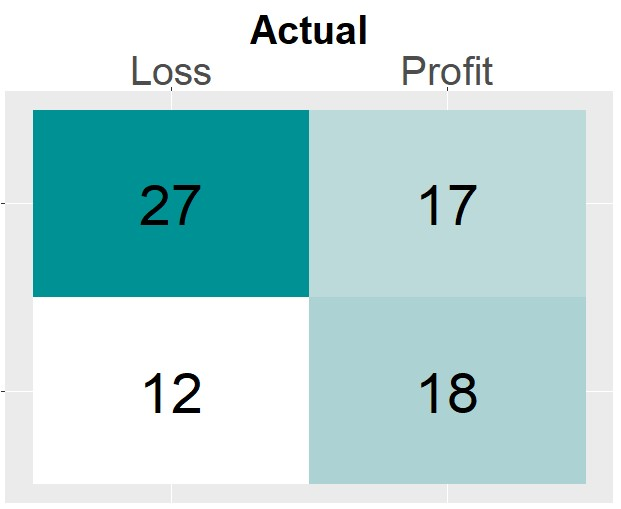
\includegraphics[width=50px, keepaspectratio]{Projekt/Figures/conf_mat_mom.jpg}\\[1cm] % Include a department/university logo - this will require the graphicx package
 
%----------------------------------------------------------------------------------------

\vfill % Fill the rest of the page with whitespace

\end{titlepage}


%%%% Indholdsfortegnelse (TOC) %%%%

\phantomsection													% Kunstigt afsnit, som hyperlinks kan 'holde fast i'
\pdfbookmark[0]{Indholdsfortegnelse}{indhold}					% Tildeler en klikbar bookmark til den endelige PDF
\tableofcontents*	
\newpage
% Here we can add figures and tables
%\listoffigures
%\newpage
%\listoftables
% Indholdsfortegnelsen (kaldet ToC) 

%\addtocontents{toc}{\protect\newpage}							% Fremtvinger sideskift i ToC hvis noedvendig (der hvor koden placeres)

\renewcommand{\cleardoublepage}{\newpage}
\mainmatter

\fancypagestyle{plain}{%
  \fancyhf{}%
  \fancyfoot[R]{Side \thepage}%
  \renewcommand{\headrulewidth}{0pt}% Line at the header invisible
}

\vspace{1.5 cm}
\selectfont



\section{Introduction} \label{sec:intro}
The global financial markets has experienced tremendous growth within sustainable investing. The mega-trend has evolved over the last two decades and incorporates an approach that emphasises corporate focus on non-financial information categorized as environmental, social, and governance (ESG) in portfolio selection. A growing societal focus on capital allocation toward sustainable investments, accountability and transparency, implies that firms cannot override infringement cases such as oil spills, accounting fraud and the use of child labor, which formerly have experienced less public attention. Furthermore, the research focus on climate change has enlightened the public and assisted a cultural shift toward a stronger focus on ESG. The escalation in sustainable investing has been institutionalized through the United Nations Principle for Responsible Investments (PRI). The PRI's long term ambition is to develop a more sustainable global financial system by encouraging and supporting signatories in incorporating the ESG factors into investment decisions. By participating in the treaty, asset managers commit to implement the financial and reporting principles for sustainable investments. The treaty has increased its number of signatories from 100 in 2006 with USD 6 trillion in assets under management (AUM) to 5.179 signatories with more than USD 121 trillion AUM \footnote{//www.unpri.org/pri.}. 

ESG objectives are becoming a primary target in asset management, where reallocation of capital has large complications for financial decision making and asset pricing. In line with increasing focus on sustainable investing, the CEO of one of the world largest asset manager, BlackRock, Larry Fink wrote in his 2020 annual letter to CEO's that his firm would exit "investments that present a high sustainability-related risk" \citep{Blackrock}. 

Understanding the relationship between SDG-related news and stock returns could provide valuable insights for investors who are looking to incorporate sustainability criteria into their investment decisions. This is particularly important as sustainable investing continues to grow in popularity, with more and more investors seeking to align their portfolios with their values. Additionally, understanding the relationship between SDG-related news and stock returns could also inform the efforts of companies and policymakers to achieve the SDGs by incentivizing companies to prioritize sustainability initiatives and enabling policymakers to design policies that support sustainable development. Therefore, investigating the relationship between SDG-related news and stock returns is not only important for investors, but also for companies, policymakers, and society as a whole.


- Massive inflow to sustainability funds
- Increased academic focus
- missing clear link
- ESG --> lower expected returns and thus a premium for sin stocks
- Some find ESG --> greater returns


- ESG ratings --> low frequency/granularity --> more difficult to use as a indicator
- ESG rating --> doesn't change very often, so difficult to use as explaining variable for returns


The growing attention towards sustainability in general has increased the focus on company specific ESG-ratings. However, ESG profiles can be difficult to

The main disadvantage of earlier research are the samples behind the results. First, the samples are often small. Second, they consist of a fixed database of news articles, which mean that they cannot be used on a daily or monthly basis to actively manage a portfolio. This thesis utilizes a database that updates on a daily basis, indicating that all new events can be captured on a daily basis.


\subsection{Motivation}

\subsection{Problem statement}

As investors increasingly consider environmental, social, and governance (ESG) factors when making investment decisions, it is important to understand the relationship between ESG-related news and stock market returns.  Specifically, does news related to the United Nations' Sustainable Development Goals (SDGs) have an impact on firms' short-term and long-term market values. The overall research questions that this thesis will investigate is the following: \\

What is the relationship between news related to the United Nations' Sustainable Development Goals and stock market returns?

To investigate this question, I have developed two main hypotheses. First, I hypothesize that news related to SDGs does not have a significant short term impact on firms' market values. The hypothesis is partitioned between positive and negative news through creation of an "a" and a "b" hypothesis.  \\

\textbf{Hypothesis 1:} 

\begin{itemize}
  \item \textbf{a.}  Negative news related to the SDGs does not have a short term impact on firm's market values.
  \item \textbf{b.}  Positive news related to the SDGs does not have a short term impact on firm's market values.
\end{itemize}

Second, I hypothesize that news related to SDGs does not have a significant long-term impact on firms' market values. \\

\textbf{
Hypothesis 2: \textit{Positive and negative news related to the SDGs does not have a long term impact on firms' market values.}}

\begin{itemize}
  \item \textbf{a.}  Negative news related to the SDGs does not have a long term impact on firm's market values.
  \item \textbf{b.}  Positive news related to the SDGs does not have a long term impact on firm's market values.
\end{itemize}


By testing these hypotheses, I hope to contribute to a better understanding of the relationship between sustainability and financial performance. 

However, I also recognize that there may be factors that influence the relationship between SDG-related news and market values. 
To explore these potential moderators, I have developed two additional sub-questions, which ultimately should expand our interpretation of the results from the main hypotheses. 

One potential moderator is the specific SDG that the news is related to. Each of the 17 SDGs represents a different aspect of sustainable development, from eradicating poverty to ensuring access to clean water and sanitation. In this regard, I will review whether the potential impact of SDG-related news on short and long term market values is independent of which specific SDG the news are related to.

Another potential moderator is the firm's level of ESG risk. ESG risk refers to the degree to which a company's operations and business practices are aligned with environmental, social, and governance principles.
By splitting the analysis on the basis of firms' ESG risk profile, I can investigate whether the impact of SDG-related news on short and long term market values is dependent on the level of ESG risk of the company. 

 
By testing these hypotheses and exploring potential moderators, I hope to gain a more nuanced understanding of how SDG-related news may impact firms' market values. Moreover, this knowledge can help investors make more informed decisions around ESG investing and encourage companies to align their business practices with sustainable development principles.


%Hypothesis 1: \textit{Negative news related to the SDGs does not have a short term impact on firm' market value.}
%Hypothesis 1a: \textit{A potential impact is independent on which SDG the news are related to.}  
%Hypothesis 1b: \textit{The potential impact is independent on the firm's level of ESG risk.}

%Hypothesis 2: \textit{Positive news related to the SDGs does not have a short term impact on firm' market value.}
%Hypothesis 2a: \textit{A potential impact is independent on which SDG the news are related to.}  
%Hypothesis 2b: \textit{The potential impact is independent on the firm's level of ESG risk.}

%Hypothesis 3: \textit{The short term impact of news related to SDGs on firms' market value is equivalent for negative news and positive news.}

%Hypothesis 4: \textit{Negative news related to the SDGs does not have a long term effect on firms market value}
%Hypothesis 4a: \textit{The potential impact is independent on the firm's level of ESG risk.}


%Hypothesis 5: \textit{Positive news related to the SDGs does not have a long term effect on firms market value.}
%Hypothesis 5a: \textit{The potential impact is independent on the firm's level of ESG risk.} 

%Hypothesis 6: \textit{The long term impact of news related to SDGs on firms' market value is equivalent for negative news and positive news.}

\subsection{Method}

\subsection{Scope and delimitation}

\subsection{Structure}


\section{Literature review} \label{lit_rev}


\subsection{A short overview of ESG and Corporate Financial Performance}

The initial mentioning of the term "ESG" has been attributed to the study "Who Cares Wins"  by the UN Global Compact in 2004 \citep{WhoCaresWins}, where the succeeding "Who Cares Wins Initiative" from 2004-2008 was built on the idea of a all-win situation for the financial industry, society and the environment. The main purpose was to incentivize the financial industry to incorporate ESG topics into their financial decision-making. The initiative was successful as the aforementioned PRI was established few years later, after which the focus sustainability in the financial world has experienced a dramatic increase. In line with the increased funding and awareness to ESG in the financial industry, the academic attention towards the issues has evolved positively as well.
According to a 1970's essay by Friedman \citeyear{friedman2007} the sole responsibility of a firm is to generate profits for its shareholders. Such a view would imply that any ESG related activity, that is not a part of the core business, should not be taken forward by the manager and neither should investors integrate information on ESG into their financial decision making.

The recent literature seems to disagree whether investing in ESG-leaders generate over-performance (alpha) in terms of returns relative to ESG-laggards. Most literature acknowledge a certain investor response to ESG initiatives, which affects the stock price, but there seems to be no clear consensus on whether the relative performance is positive, negative or simply explainable by other factors. 

\cite{ESG_meta_analysis} made an meta-analysis of more than 2.000 studies looking into the potential of ESG investing. The results of the studies differ depending on which ESG methodology (e.g. source and granularity) were used and which financial metrics were applied (e.g. return or exposure to Fama-French factors). They conclude that the majority of studies find stable positive ESG impact on performance over time. However,  once screened for portfolio performance, such as transaction costs, the studies reporting a positive correlation decreases. 


Although the evidence of negative correlation between ESG-activities and CFP is limited, the theoretical foundation is supported by the aforementioned statement from Friedman and the efficient market hypothesis. If the market is partly driven by socially responsible investors that screen out low-ESG assets, then one would theoretically observe negative correlation between sustainable investments and CFP, and investors would pay a premium for their preference for sustainability. 


Some empirical studies give reason to doubt an optimistic view on a firm's ESG activities, providing evidence for financial costs for companies from being proactive in ESG matters. 

For example \cite{ESG_Frontier} integrates ESG characteristics in the portfolio construction of the efficient frontier instead of as a screening factor. They quantify the cost of ESG preferences as the drop in Sharpe ratio when choosing a portfolio with better ESG characteristics than the efficient portfolio. The authors find that integrating the ESG preferences by a proxy for governance, the maximum Sharpe ratio is achieved for a high level of ESG, implying that ethical goals can be done at little cost. Imposing constraints will always reduce the Sharpe ratio for any given ESG score. The proxies for E, S and overall ESG are weaker predictors of future profits. 

Moreover, the findings from \citep{uk_ESG_stock} show that companies with higher social performance scores exhibit minor returns than those with lower social performance scores. They state that social performance indicators are negatively related to stock returns and that abnormal returns are available from holding a portfolio of the socially least desirable firms. In addition, \cite{Kacperczyk_sin_stocks} advocate that so called "sin stocks"\footnote{Classified as companies involved in alcohol, tobacco, gambling or the weapons industry. } have higher expected returns than stocks of otherwise comparable characteristics, due to them being neglected by constrained investors. Negative screening will lead to these stocks being under-priced in relation to fundamental value.   

For example, using yearly sustainability ratings \cite{Shrunk_ESG_ALPHA} address the question whether non-financial information in ESG scores offers additional performance benefits by construct long-short ESG strategies and asses their value-added to investors. They find that claims of ESG out-performance only hold when considering isolated returns. However, when applying standard risk adjustments, the strategies perform like simple quality strategies constructed from accounting ratios. 


Supporting the evidence from \cite{ESG_meta_analysis}, the paper from \cite{factor_ESG_integration} investigates the impact of ESG integration on different factor-investment strategies. Their results show that a manager of a factor portfolio can increase the portfolio exposure towards ESG intensive companies without impairing the exposure toward the desired factors, such as value and low volatility. For example, the minimum volatility strategy only experienced a 7\% reduction in factor exposure from a 30\% increase in exposure to ESG. The results suggest that investors would be able to improve the ESG characteristics of their portfolio without harming their ability to capture market returns. 

Similarly \cite{ESG_exposure_approach} finds averagely positive ESG return premia between 2009 and 2020. They utilize an exposure-matching approach to isolate and measure the return premium related to ESG by neutralizing the exposure to other factors. The benefit is that they are able to control for risk and sector differences to measure month-on-month ESG returns. They also discuss the advantages of using their approach over a regression approach that sorts stocks into portfolios given ESG attributes, but mainly state that it is of more practical use whereas the latter is more useful within academia.

Additional research acknowledge an investor response to firm's ESG activities which affects the companies performance in different ways (\cite{lins2017social}; \cite{kim2014corporate}; \cite{el2011does}). These studies use yearly observations and explain their findings by concepts of trust-building in sustainable activities, which facilitates the firm to obtain benefits such as lower cost-of-capital, lower crash risk, higher and long-run profitability.

The insights from these findings dictate various long-term benefits of both investors and firms from engaging in ESG intensive investment activities. It is relevant to assume that these benefits are particularly suitable for long term investors in diversified portfolios, whereas short term investment strategies will require information on a more granular basis than yearly ratings, when implementing ESG factors into their investment decision. Applying yearly observations ignores the changing landscape of the market, where news are spreading promptly over the internet. Moreover, the potentially impulsive behavior of a large group of speculators and retail investors, who might base their decisions on instant new information becoming available, as per \cite{black1986noise}. Capitalizing on the possibilities of looking beyond yearly data points may add more insights into whether investors incorporate ESG-related information into their financial decision making \citep{Sustainable_sentiment}. 

Increasing the granularity of observations can be done by relying on public news articles, with a focus on ESG-related matters, as a proxy for ESG engagement of companies. 

- Sustainable investing with ESG rating uncertainty

\subsection{Relevant sentiment analysis literature}


Our approach evolves around a popular core of literature that links public sentiment, through news articles, with financial performance on the stock market. Two of the early comprehensive publications are \cite{tetlock_sentiment} and \cite{baker_sentiment}. \citeauthor{tetlock_sentiment} shows that high media pessimism predicts downward pressure on stock prices followed by a reversion to fundamentals. \citeauthor{baker_sentiment} studies how investor sentiment affects stock returns. Their main empirical finding is that future stock returns are conditional on beginning-of-period sentiment. That is, when sentiment is high, stocks that are attractive to speculators - small stocks, unprofitable stocks, high-volatility stocks and more - tend to earn relatively low subsequent returns, while if sentiment is low these stocks earn relatively high returns.   

\cite{Blancard_ESG_sentiment} utilize the ideas from the aforementioned authors to investigate the relationship between positive and negative ESG news and changes in firm market value. They conduct an event study and find that investors on average react negatively to negative events, while positive events has no impact. 

We want to elaborate on the relation between sustainability of firms and financial performance, by combining the ideas from the previous sections on ESG and sentiment analysis. We will focus on news articles that contain company specific information in relation to the United Nations Sustainable Development Goals\footnote{https://www.un.org/development/desa/disabilities/envision2030.html} (SDGs), and research how company valuation responds to such events. 



\subsection{Market theory}




\subsection{Identification of gap in the literature}




\section{Methodology and theory} \label{sec:method}
\subsection{The Event Study Methodology}

The short-term event study examine the behavior of stock returns around corporate events, and is used to measure shareholders' reaction to unexpected news. 
- Something with Fama


\subsection{The Market Adjusted Model}

In the context of event studies, an expected return model is a hypothetical prediction of the stock return. The individual stock price return is measured against the market return, as a simple way to control for potential effects of the event on the general market. The model does not adjust for basic CAPM risk and thus abstracts from the individual firm's distinct risk profile. The argument for implementing a simple model is to give a general overview of long and short term return-effects from events, and not to provide statistical conclusions. 
The daily excess returns are measured as the difference between the stock return and the market return on a given day, with the market return assumed to be the MXWO\footnote{https://www.msci.com/World} index:
\begin{equation}
    \text{Abnormal Returns} \:  (AR_{i,t}) = R_{i,t} - R_{M,t} 
\end{equation}
Where, $R_{i,t}$ is the return of stock \textit{i} on day \textit{t}, and $R_{M,t}$ is the return of the market on day \textit{t}. 

The returns series for stock \textit{i} is indexed wrt. the event date (t = 0) by setting the value to 100 and expressing the cumulative return of the future and foregoing observations with respect to this value, to isolate the effect of the event from the discrete trading days. 

The argument is that on t = 0 the information becomes available to the market. However, the investor will not be able to trade on the information before the following trading day. The return index is calculated as the 
cumulative product of the daily excess return leading up to or following the event date multiplied by 100. 

\subsection{Short-term abnormal returns}

The inspection of short-term abnormal return behavior covers (2n+1) trading days surrounding a corporate event: n days before to catch possible insiders information, the day of the event, and n days after. The short term analysis will use N = 10, which leaves a total window of 21 days [-10,+10] to investigate effect from an event. The effect of an event is expressed in terms of the abnormal return, defined as the difference between the realized ex-post return and the expected return, with the latter characterized as the expected return conditional on the event not taking place \citep{Event_studies}. Several models have been applied in the literature to estimate the short-term abnormal returns in event studies, which includes the CAPM, the Market Model, and multi-factor models. According to \cite{holler2014event} the most widely used is the Market Model, which assumes a linear relationship between the individual stock return and the market return. 

\subsubsection{The Market Model}

The Market Model is a single factor statistical model, which relates the return of a given security to the return of the market portfolio. The linear specification follows from the assumed joint normality of asset returns. For any given stock the model is defined as:

\begin{equation} \label{market_model}
    R_{i,t} = \alpha_i + \beta_i * R_{m,t} + \epsilon_{i,t},
\end{equation}
 where $R_{i,t}$ is the return of the stock \textit{i} on day \textit{t}, $\alpha_i$ is the regression intercept\footnote{The excess return of a stock relative to the market, that is not explained by the $\beta$.} for stock \textit{i}, $R_{m,t}$ is the market return on day \textit{t}, and
 $\beta_i$ is the sensitivity of $R_{i,t}$ to the market return.  

 The regression coefficients $\alpha_i$ and $\beta_i$ are computed as the stock returns of a given frequency on the market returns. To analyze the market participants' short-term reaction before and after the event date, the event window is set to +-10 days around the event date, and the estimation window of the regression is set to 120 days prior to the event, as proposed by \cite{Event_studies}. The linear ordinary least squares (OLS) has been applied in the estimation. \cite{brown1985using} investigate the properties of applying daily stock returns in event studies with the market model, and find that the model is well-specified under a variety of conditions. 

 With the expected returns predicted from the Market Model, the abnormal returns are defined as the residual between the realized and the expected returns for each event:
 \begin{equation}
     AR_{i,t} = R_{i,t} - (\alpha_i + \beta_i * R_{m,t})
 \end{equation}

 where $AR_{i,t}$ measures the shareholder's reaction to the event addressing firm \textit{i} at time \textit{t}  with $\alpha_i$ and $\beta_i$ defined as the OLS-parameter estimates from the regression in equation \ref{market_model}. The abnormal return can be transformed into average, cumulative, and cumulative average abnormal returns (for n = (1, ..., 10) by: 
  \begin{equation}
     AAR_t = \frac{1}{N} \sum_{i=1} ^{I} AR_i
 \end{equation}
 \begin{equation}
     CAR_{i,t}[-n,+n] = \sum_{\tau = t-n} ^{t+n} AR_{i,t}
 \end{equation}
 \begin{equation}
     CAAR_{[-n,+n]} = \sum_{\tau = t-n} ^{t+n} AR_{i,t}
 \end{equation}
 
 The AAR is the average of the AR per time period, the CAR is the cumulative sum of the AR per stock, and the CAAR is the cumulative sum of the AAR of all stocks and over windows. 



 

\subsection{Long-term abnormal returns}

\subsubsection{Portfolio sorts / Calendar Time Portfolio Approach}








\section{Empirical results} \label{sec:analysis}

\subsection{Data description}


\subsection{Estimation methodology}

\subsection{Abnormal returns in the market adjusted model}


\subsection{Short term abnormal returns in the Market Model}

To test hypothesis #1 and #2 of whether negative and positive SDG related events impacts firm value on the short term, we set apart negative and positive events and assess the aggregated development in abnormal returns 10 days before and 10 days after an event. Moreover, we isolate the effect of the individual SDGs to test hypothesis #4 of whether events on some sustainability goals are more relevant for investors than other. We apply the Market Model to measure abnormal returns around an event.   



\subsubsection{Negative news}

The average abnormal returns and development in cumulative average abnormal returns calculated from the Market Model are illustrated on aggregate in figure \ref{fig:ST_neg_news}. To support the analysis, the AAR and CAAR are portrayed along with their respective 95\% confidence intervals and the amount of events on a given day relative to the event date $(t = 0)$ (right y-axis) represented by the barplot in the background. 

The left y-axis depicts the abnormal return and the x-axis is the number of days before and after an event has occurred. The effect of negative events on average stock behavior is represented by the blue line in the graph, and is mostly negative leading up to an event. The impact from negative events is approximately zero until $t = -6$ upon which the AAR decreases steadily until the event date, where it bottoms at $-0.36\%$. After a negative event at $t=0$ the AAR increases, however still negative until $t=2$, towards neutrality at zero and remains there for the rest of the window. The CAAR stays negative during the full event window and bottoms on $t=2$ after a large decline of approximately $1.2\%$ from  $t=-5$. Moreover, the AAR is significantly negative between $t=-2$ and $t=0$ at $95\%$. The same goes for the CAAR after $t=-2$ and the remaining window. Generally, negative news seems to be priced in leading up to and including the identified event day, after which they have limited impact. \\ 
The bars offers insights into the extent of observations leading up to an event. The bars begin to increase at $t=-5$ at which the AAR begins to decline, which imply a relation between attention towards negative news and pessimistic investor behavior even before the event date. Furthermore, this is an indication that the specified event time may be lagging the incident of the *true* event, which is a disadvantage of this model setup. 

\begin{figure} [H]
    \centering
    \caption{Negative news: $CAAR_{t=10}$}
    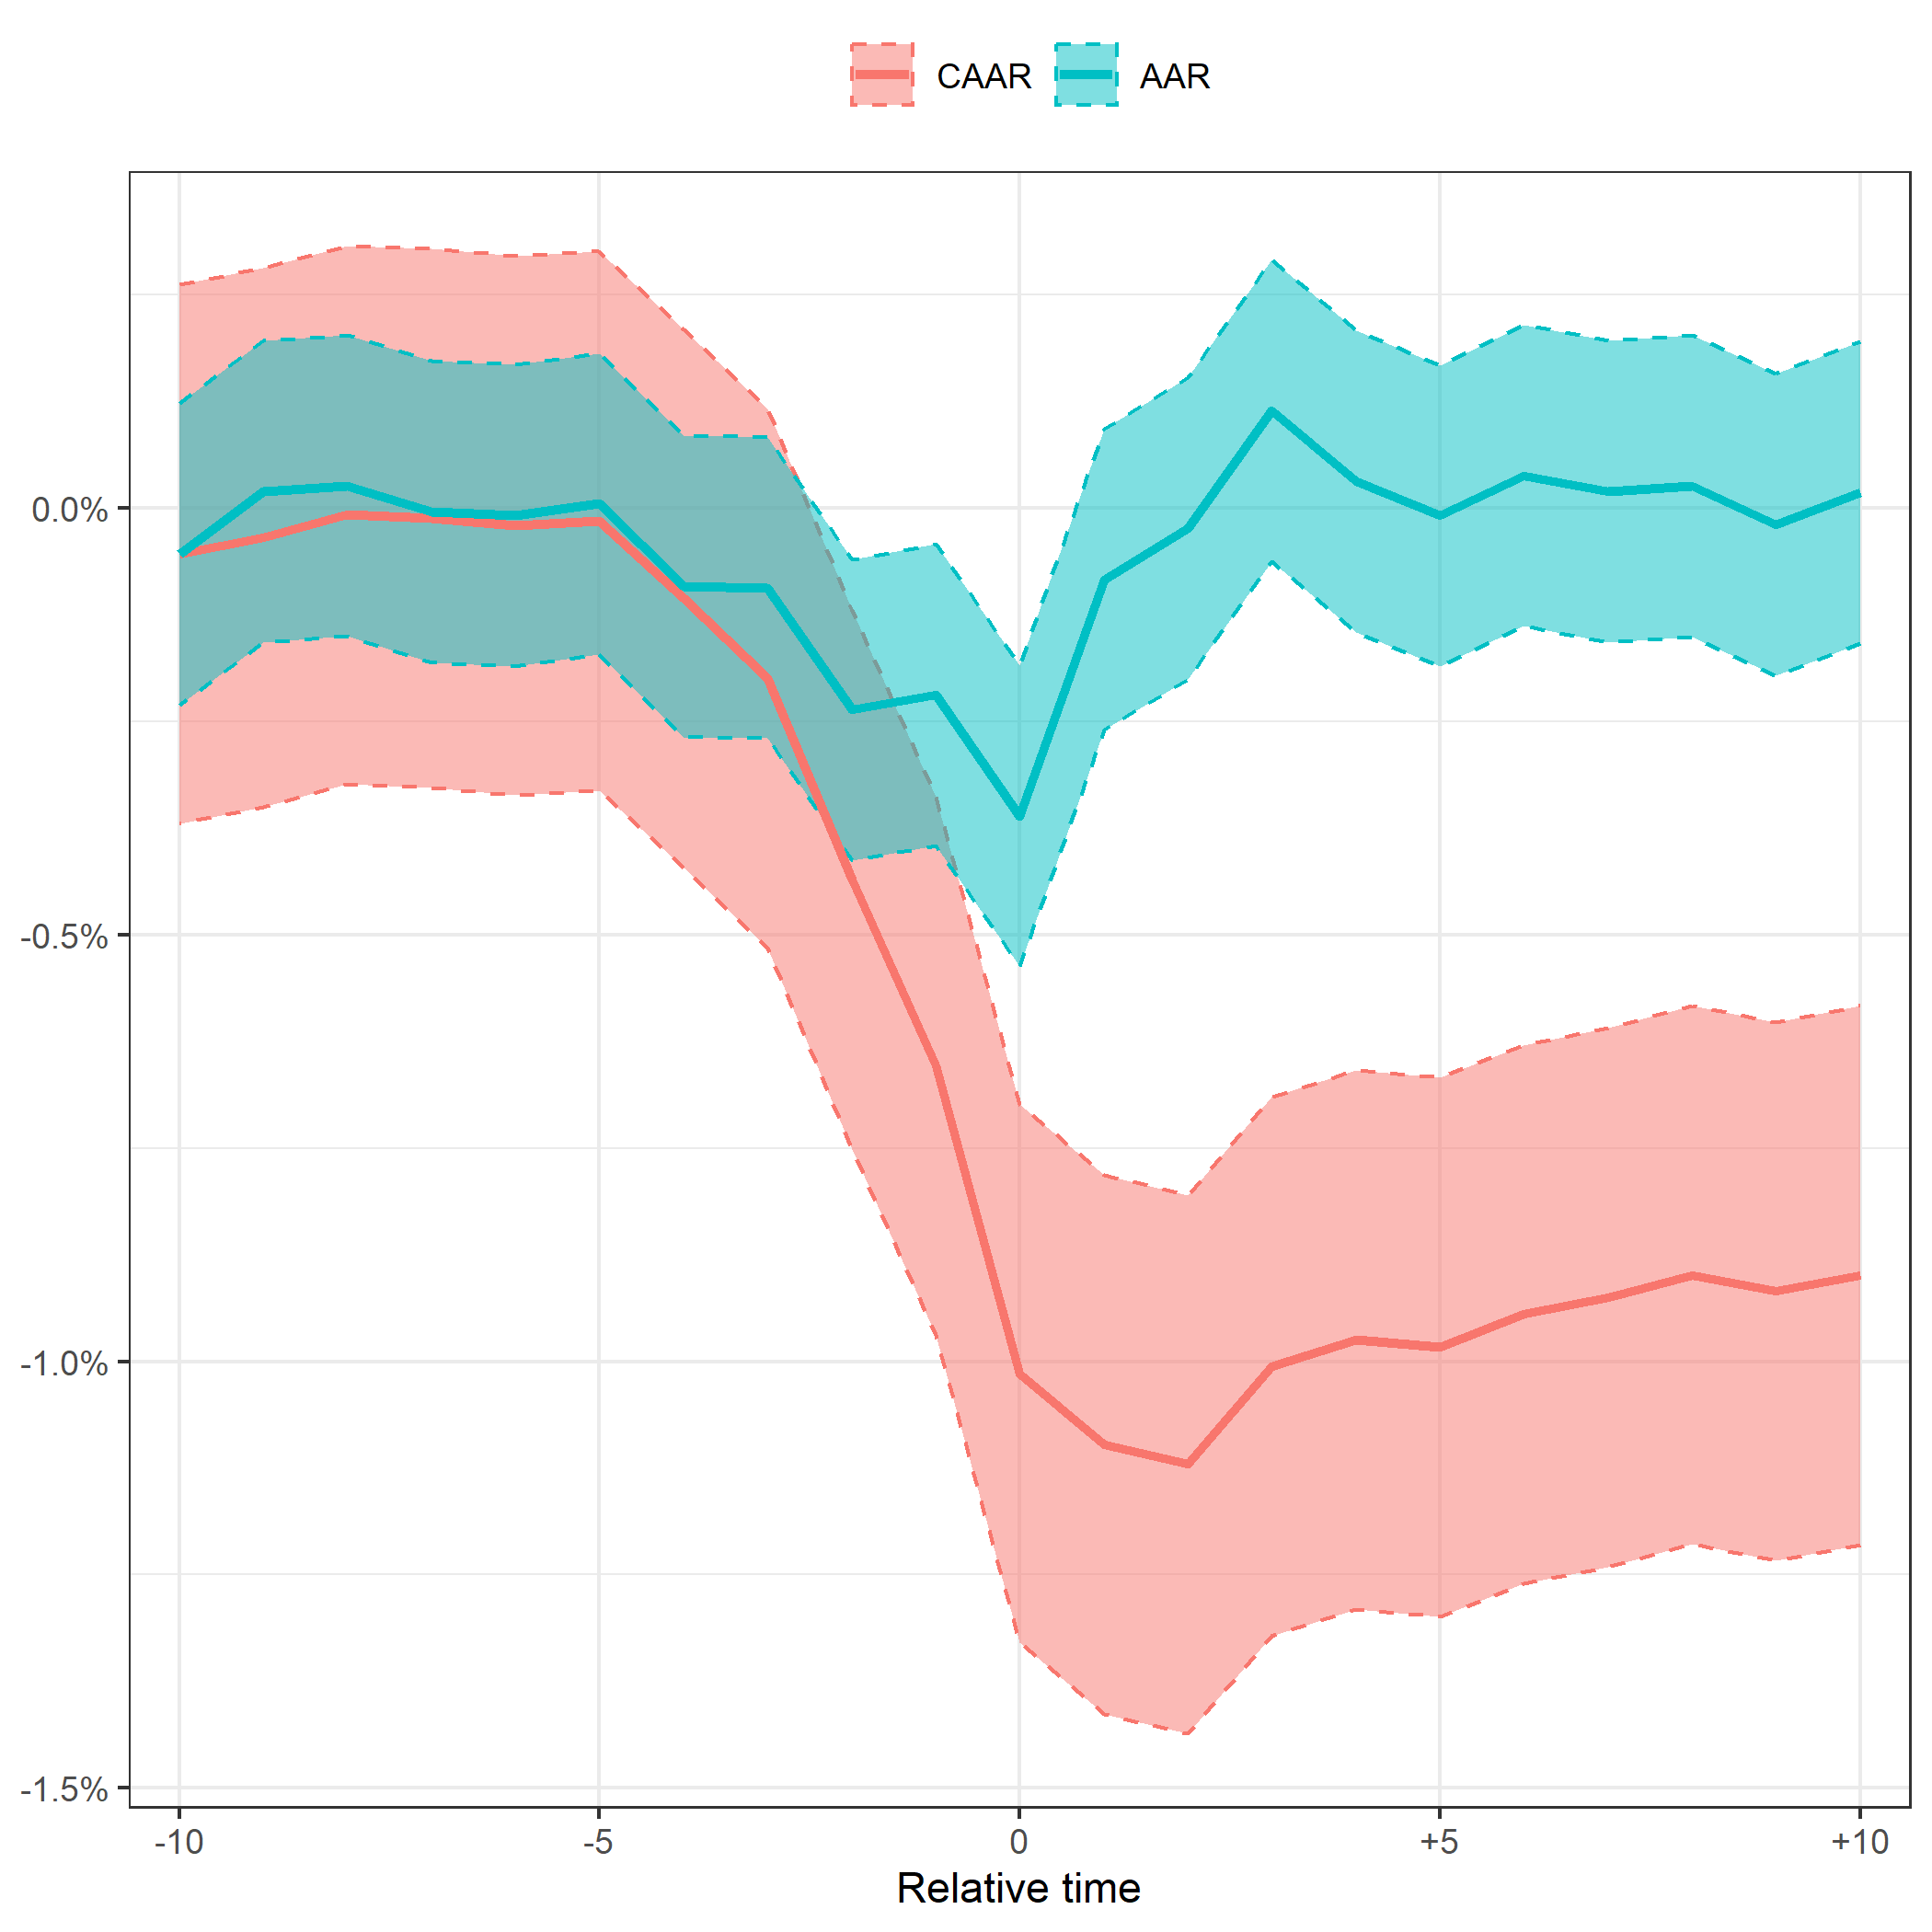
\includegraphics[scale=0.6]{Projekt/1.Figures analysis/ST_negative_all_CI.png}
     \caption*{\footnotesize The figure illustrates the average abnormal return (AAR) and cumulative AAR (CAAR) around the event date (t = 0) of negative news. The lines (left axis) represent the average and the ribbons represent the 95th confidence intervals. The bars (right axis) represent the amount of events on a given day relative to t = 0. }
    \label{fig:ST_neg_news}
\end{figure} 

Examining the average effect from, respectively, positive and negative events provides insights into the overall tendency of the relation between shareholder sentiment and corporate sustainability. By investigating the abnormal returns resulting from events specific to the individual SDGs one can gain a deeper understanding of which themes within corporate sustainability that investors places most emphasis with. Figure \ref{fig:ST_neg_bar} illustrates the aggregated CAAR over the full event window (from $t=-10$ to $t=10$) from events related to specific SDGs along with corresponding confidence intervals. 

\begin{figure} [H]
    \centering
    \caption{SDG 5 pillars: negative news}
    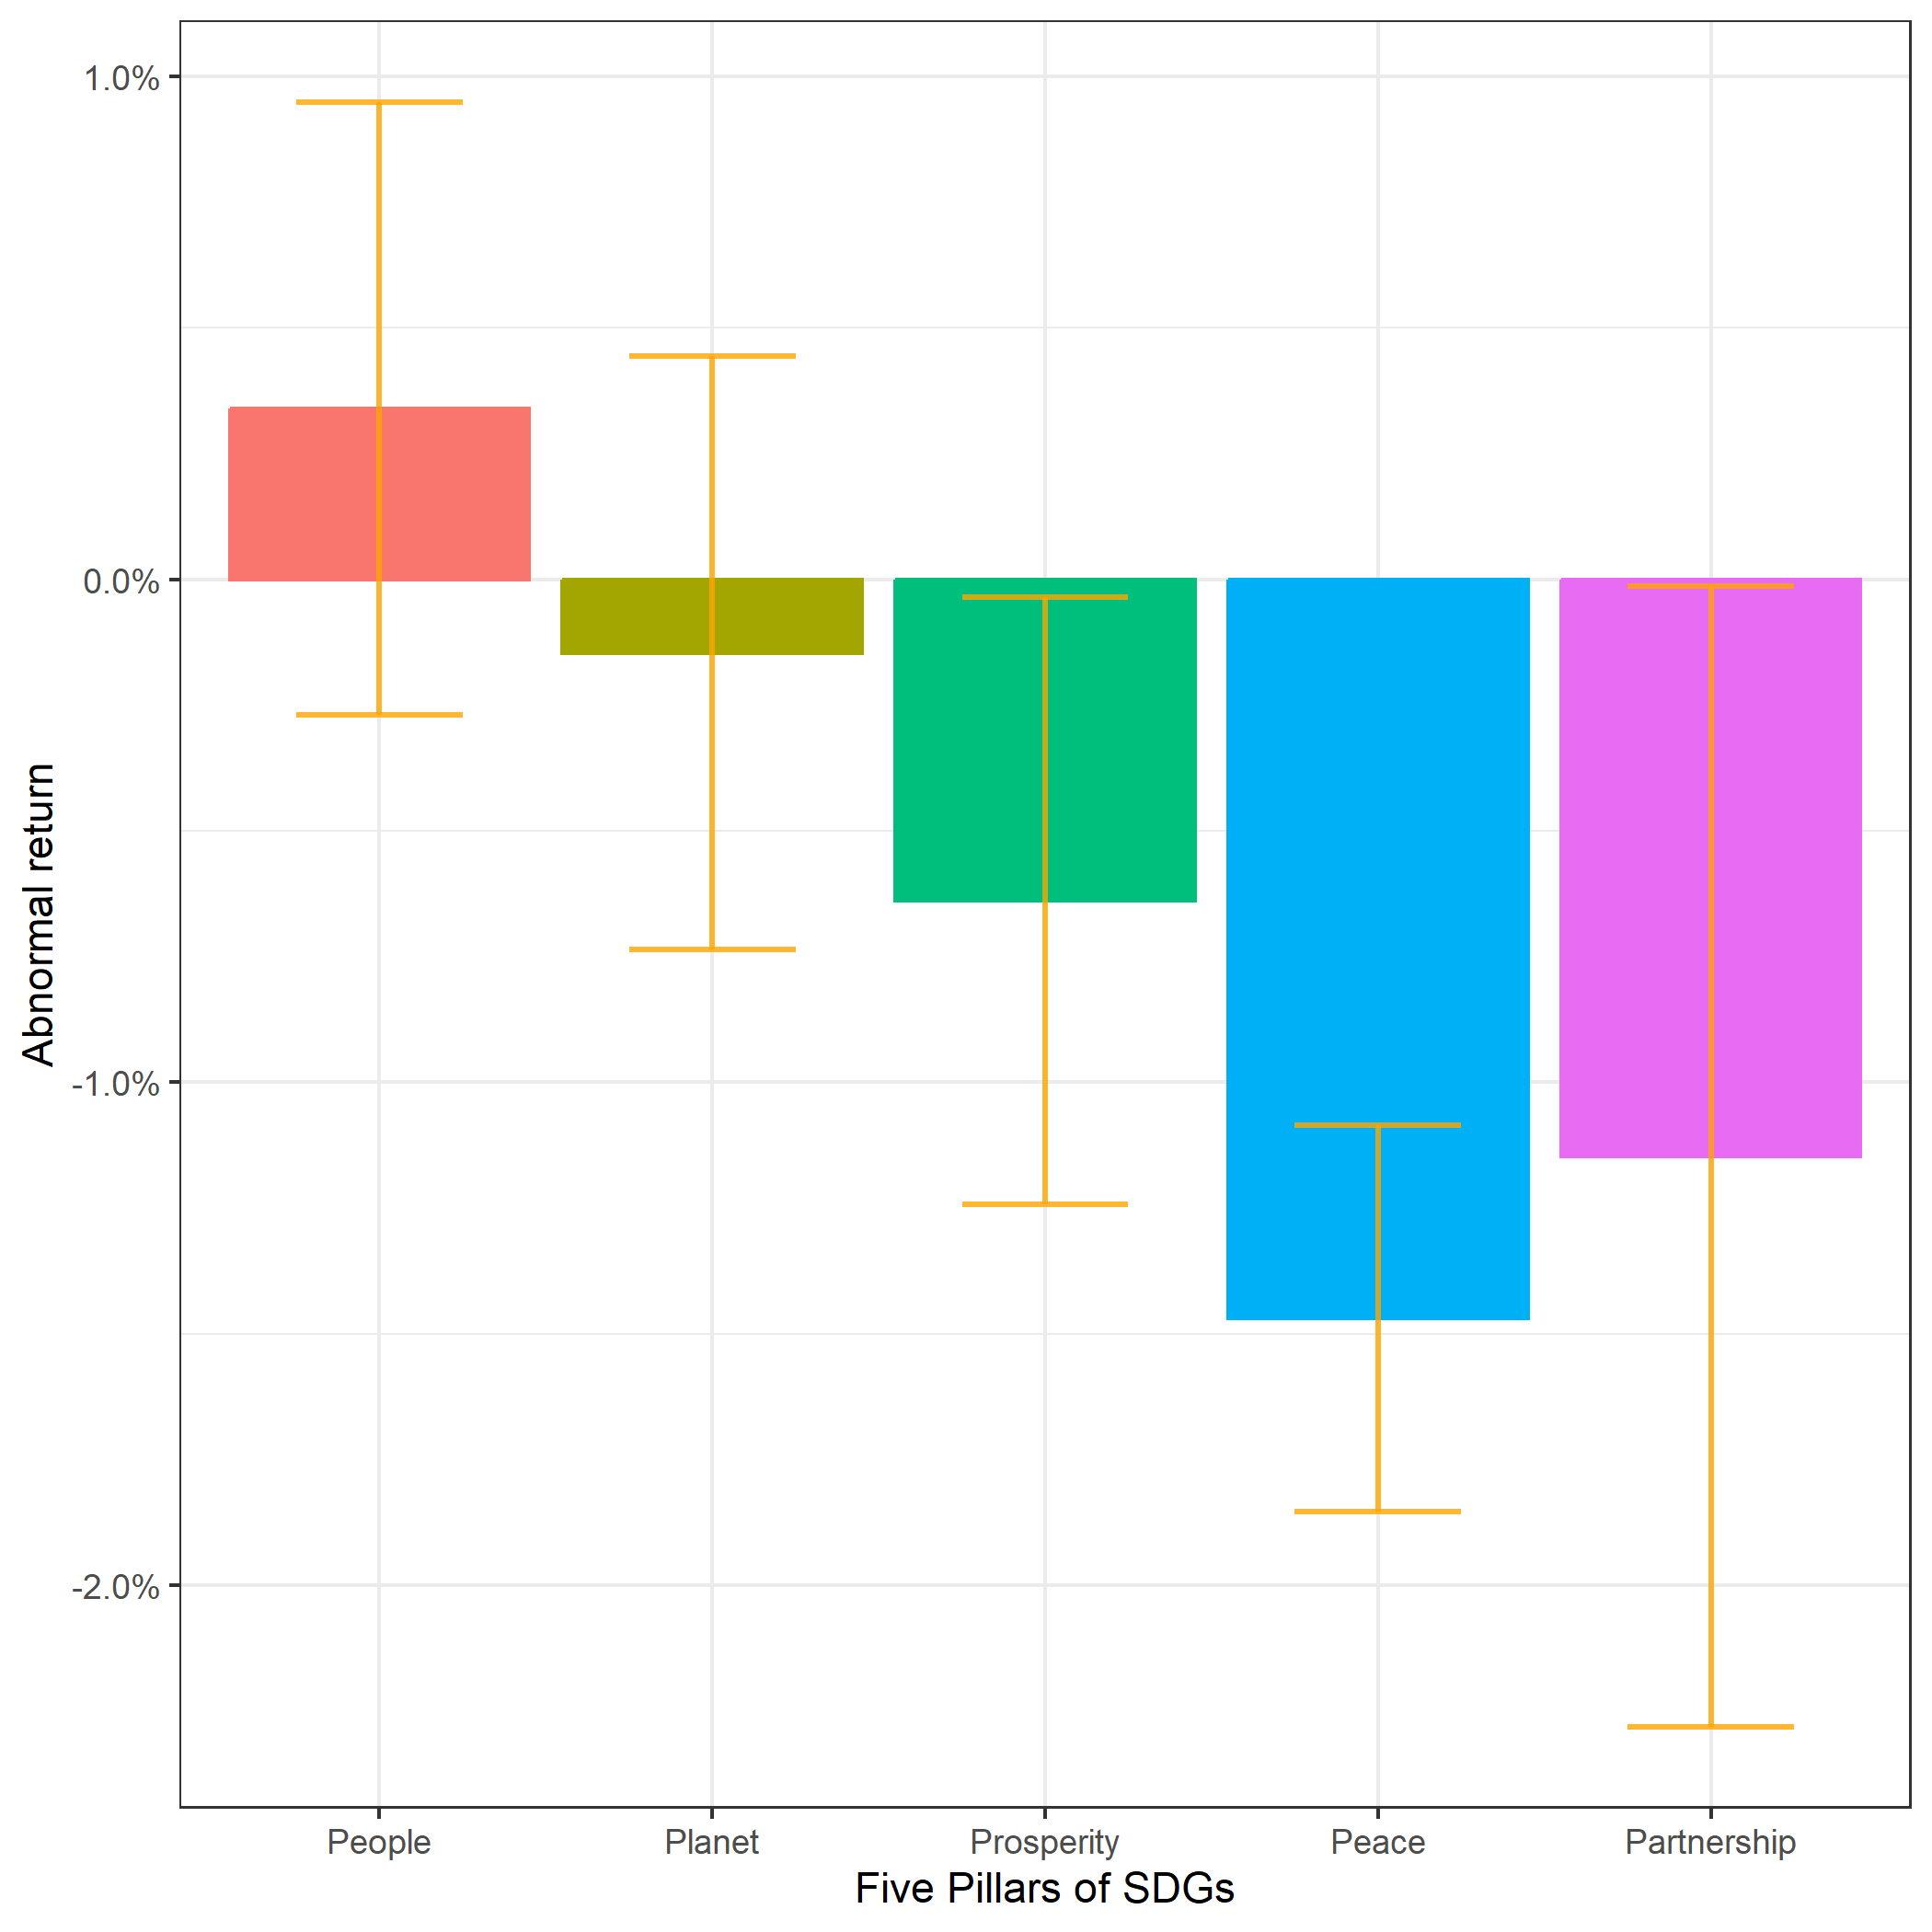
\includegraphics[scale=0.6]{Projekt/1.Figures analysis/ST_negative_sdg_bar_groups_0.png}
    \caption*{\footnotesize The figure illustrates the CAAR on $t = 10$ (the full period) from negative news. The error bars represent the 95\% confidence intervals of the CAAR.}
    \label{fig:ST_neg_bar}
\end{figure}

Splitting the events on SDGs generally illustrate that negative events in most groups are associated with negative abnormal returns. However, the issue of statistical uncertainty in the measurements means that one cannot generate a lot of insights from the aggregated values. Only SDG 15 and 16 provides abnormal returns significantly different from zero. The statistical uncertainty originates from the relatively low amount of observations associated with the individual groups after dividing the events into SDGs. For example, SDG 4 and 9 has only, respectively, 16 and 83 observations, which results in a vast excessively wide confidence interval, whereas SDG 12 and 16 has, respectively, 576 and 1364 observations, and correspondingly very narrow error bands. 

The significance of the results in relation to negative and positive events are summarised with a z-test in table \ref{tab: ST_significace}, which presents the z-scores and significance complementary to the AAR on $t=0$, along with the CAAR on respectively, two, five, and 10 days around the event.  



The selection method for negative events was proposed to gather cases of severe negative abnormal returns. The CAAR of the full and subset windows from negative events are significantly different from zero at $p \; < 0.01$, which further validates the selection method and that negative abnormal returns are attainable to negative events. However, the method may be late to pick up the signal of negative events or new information on the market.  

\begin{table}[ht]
\centering
\caption{AAR and CAAR over event window (in percentage)} 
\begin{tabular}{lllll}
   \hline  \hline
  & $AAR_{t=0}$ & $CAAR_{[-2;+2]}$ & $CAAR_{[-5;+5]}$ & $CAAR_{[-10;+10]}$  \\
 \hline
Positive news & $\underset{(1.973)^{**}}{0.073}$  & $\underset{(-0.211)}{-0.016}$    & $\underset{(-0.379)}{-0.043}$ & $\underset{(-1.091)}{-0.164}$  \\ 
Negative news & $\underset{(-3.457)^{***}}{-0.360}$  & $\underset{(-5.749)^{***}}{-0.917}$    & $\underset{(-4.761)^{***}}{-0.955}$ & $\underset{(-3.288)^{***}}{-0.888}$  \\ 
   \hline
   \multicolumn{5}{p{12cm}}{\footnotesize  $^* \; p\; <\; 0.1$, $ ^{**} \; p\; <\; 0.05$, $ ^{***} \; p\; <\; 0.01$  } \\ 
\end{tabular}
\label{tab: ST_significace}
\end{table}

\subsubsection{Positive news}

According to figure \ref{fig:ST_pos_news} the identified positive events doesn't seem to be associated with any significant reaction from the shareholders on average, as the AAR doesn't fluctuate significantly from zero during the event window besides a marginal deviation at the event date. Following, the statistical uncertainty of the CAAR becomes more widespread through the event window, as indicated by the widening red ribbon. The negative tendency of the CAAR is insignificant since the measure is based on, likewise, insignificant AARs, meaning that one cannot for certain state that the cumulative effect is different from zero. 

\begin{figure} [H] 
    \centering
    \caption{Short term positive news: AAR and CAAR}
    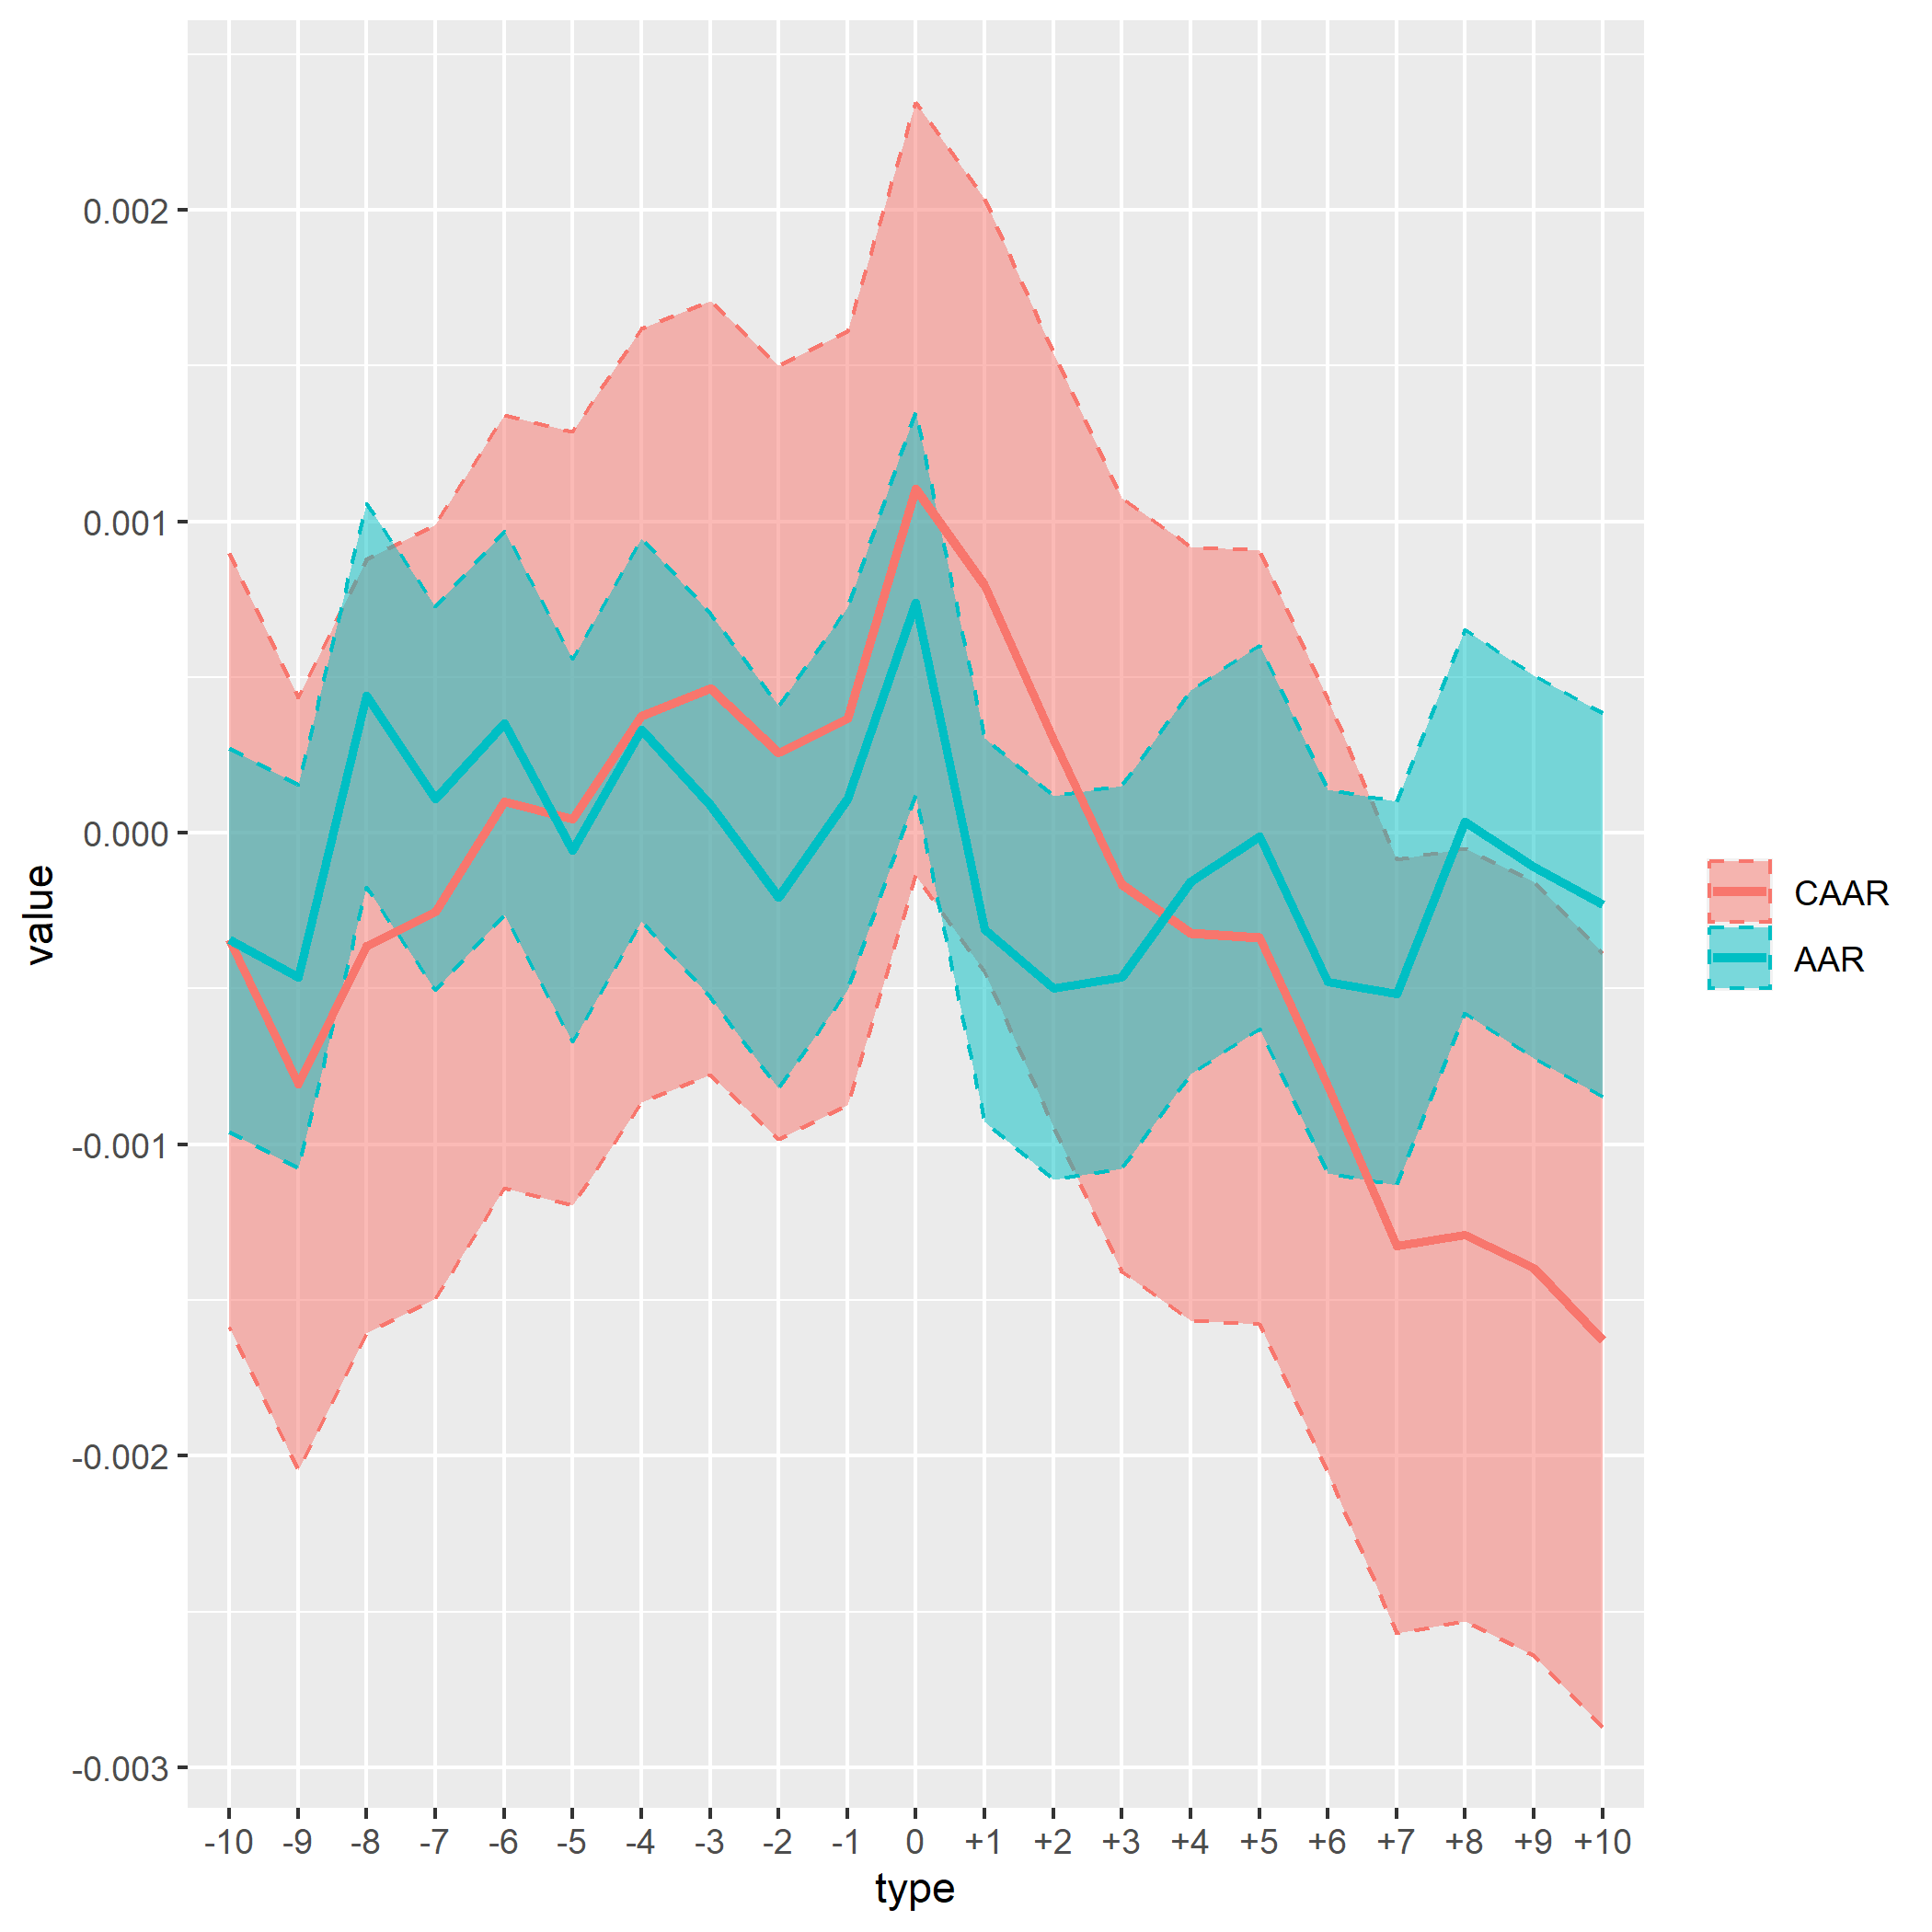
\includegraphics[scale=0.6]{Projekt/1.Figures analysis/ST_positive_all_CI.png}
    \caption*{\footnotesize The figure illustrates the average abnormal return (AAR) and cumulative AAR (CAAR) around the event date (t = 0) of positive news. The lines (left axis) represent the average and the ribbons represent the 95th confidence intervals. The bars (right axis) represent the amount of events on a given day relative to t = 0. }
    \label{fig:ST_pos_news}
\end{figure}


The tendency of insignificance related to positive events is further reinforced by the results from the individual SDGs, as most are statistically indistinguishable from zero. However, the aggregates do indicate that positive events on SDGs in general are associated with negative abnormal returns. In contrast to the case of negative events, where the main issue was the amount of observations, the underlying issue with uncertainty comes with the seemingly random shareholder reaction to positive events. 
 
\begin{figure} [H]
    \centering
    \caption{SDG 5 pillars: positive news}
    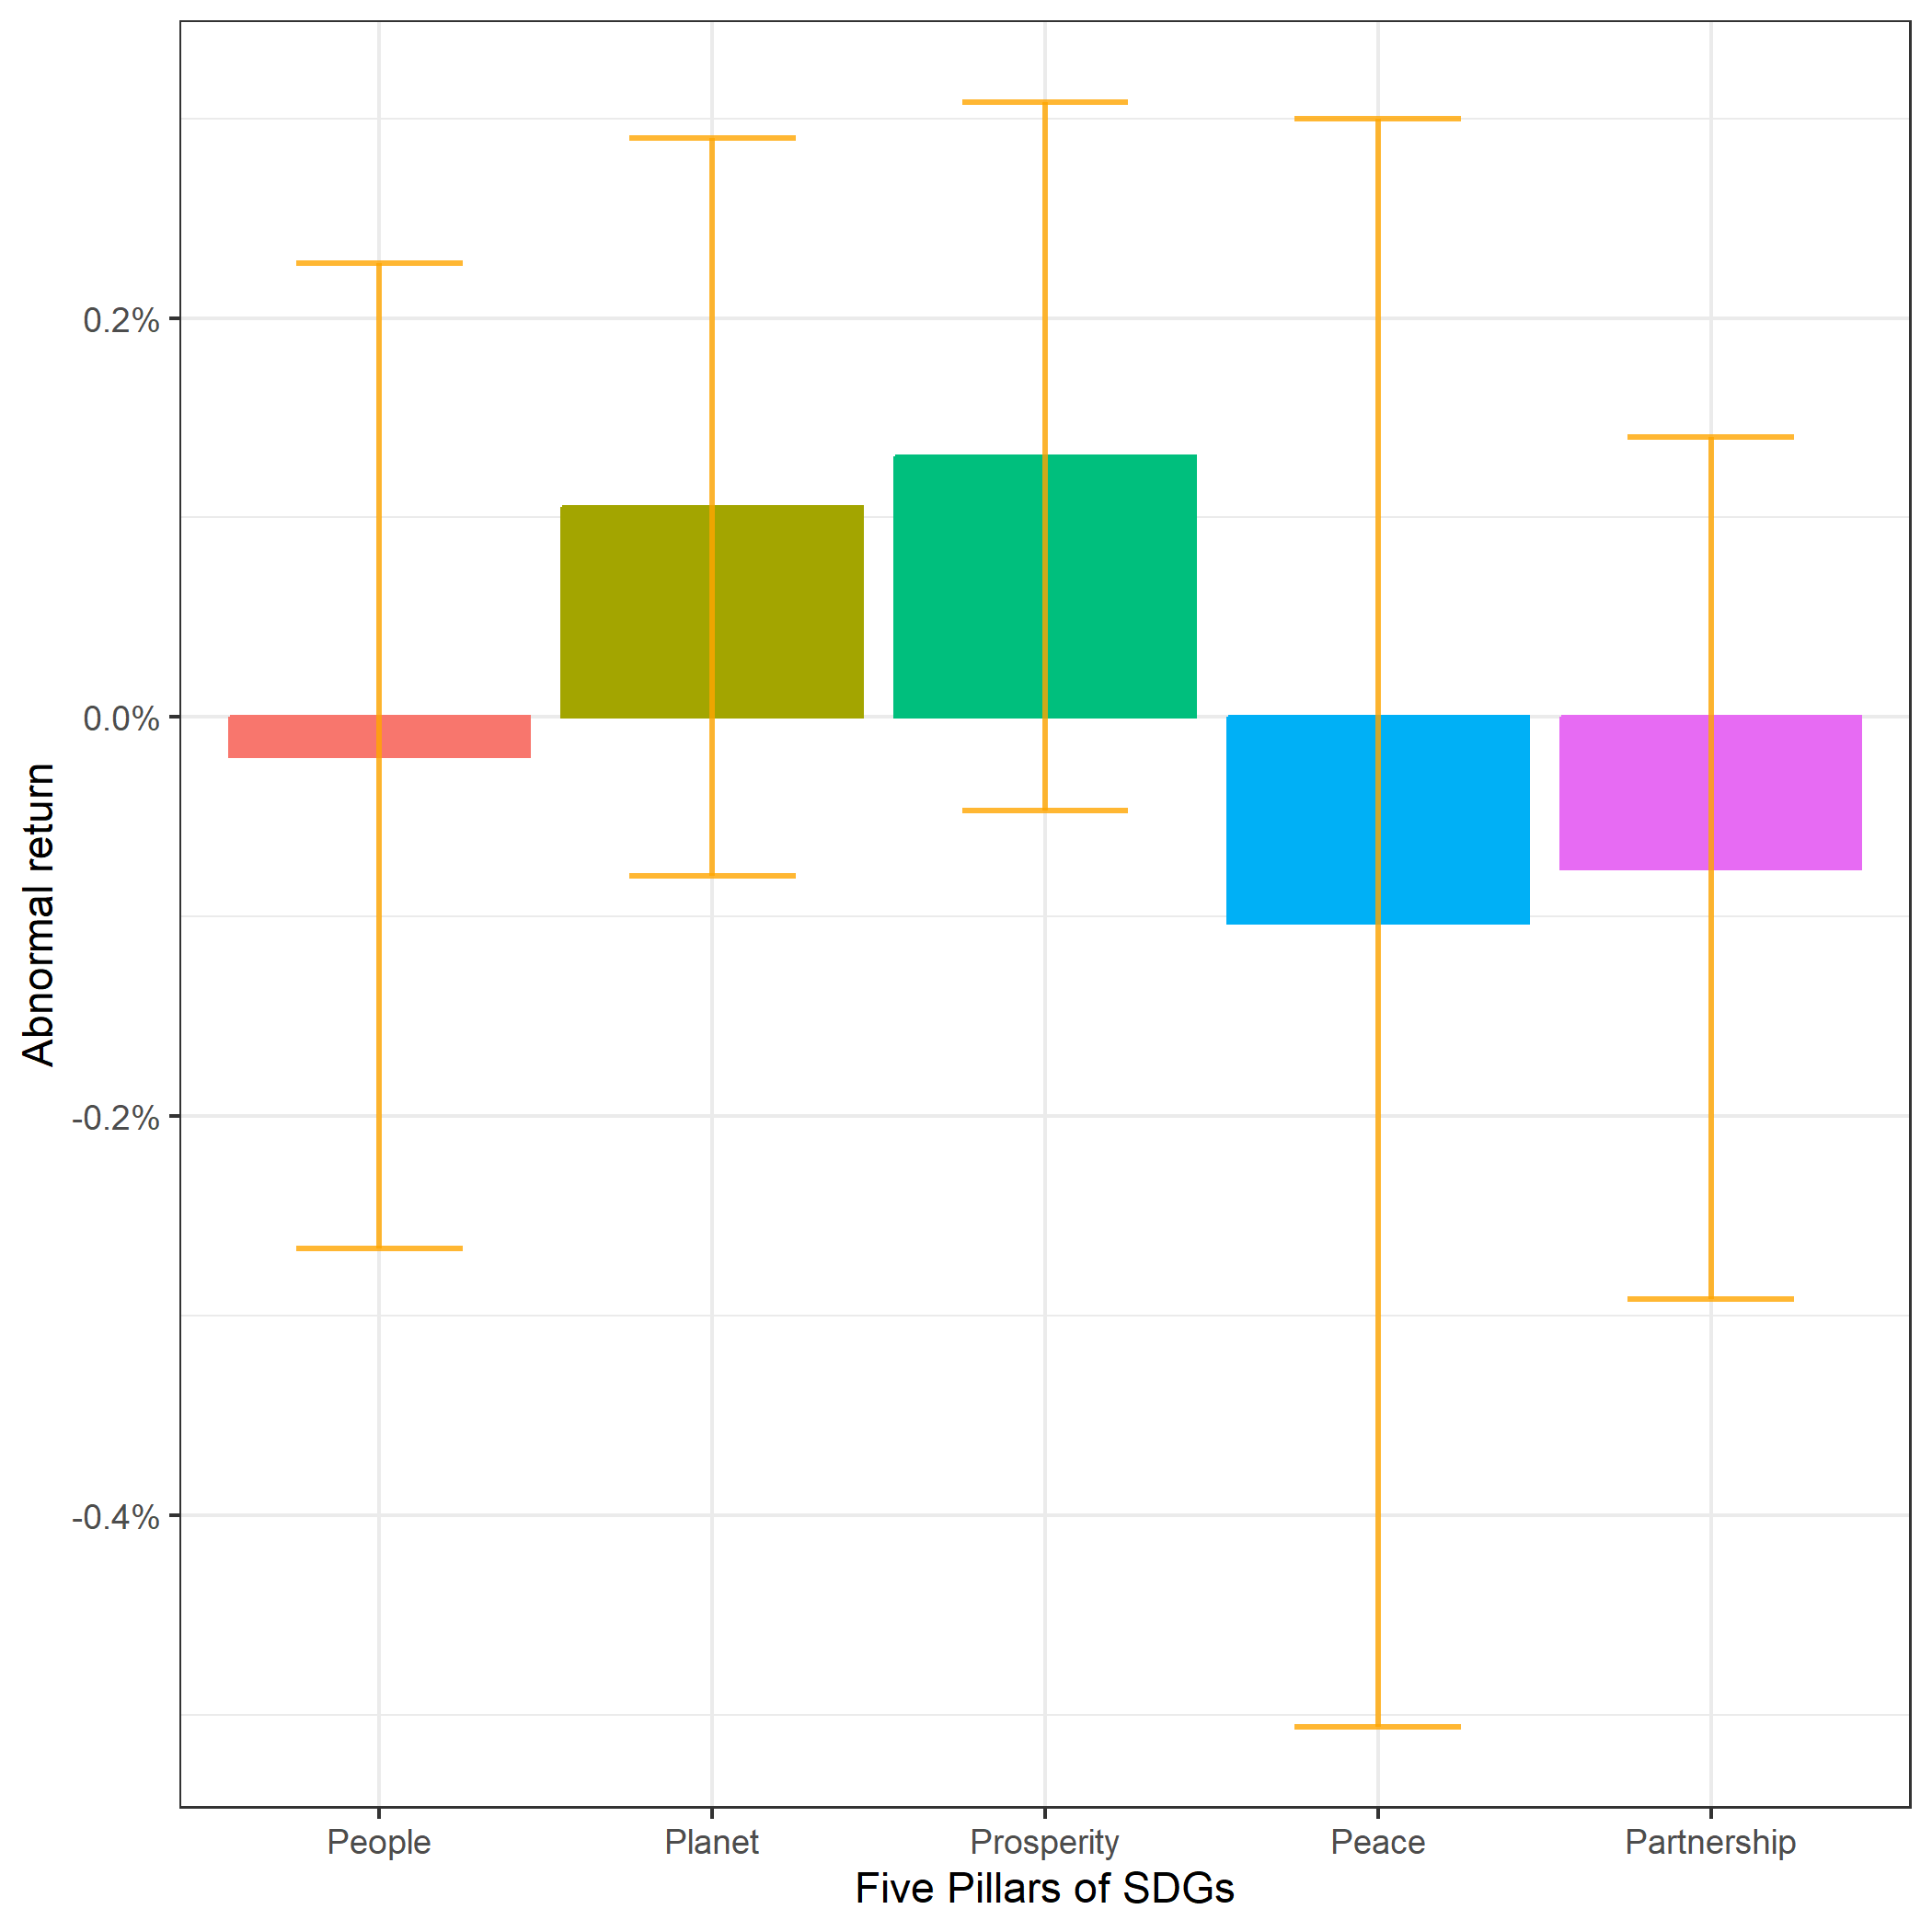
\includegraphics[scale=0.6]{Projekt/1.Figures analysis/ST_positive_sdg_bar_groups_0.png}
    \caption*{\footnotesize The figure illustrates the CAAR on $t = 10$ (full period) from positive news. The error bars represent the 95\% confidence intervals of the CAAR.}
    \label{fig:ST_pos_bar}
\end{figure}

The insignificance of the abnormal returns associated with positive events are manifested in table \ref{tab: ST_significace}. The the CAARs on, respectively, two, five and 10 days around the event are all insignificantly different from zero. In contrast the AAR exhibit positive performance at $t = 0$ at 5\% significance. 

Generally, the short term empirical evidence demonstrate a non-verifiable relation between positive events, related to both broad and specific SDGs, and abnormal returns. Positive news is however associated with an instant reaction from investors on the event date. The evidence point towards an overall negative relationship, but this is not statistically valid.  


\subsection{Long term abnormal returns}

\begin{table}[]
\begin{tabular}{llllllll}
\hline \hline
\textbf{} & \multicolumn{3}{c}{FF-3 Factor} &  & \multicolumn{3}{c}{FF-5 Factor} \\ \cline{2-4} \cline{6-8} 
          & 1 sd       & 2sd     & 3 sd     &  & 1 sd      & 2sd      & 3 sd     \\ \cline{2-4} \cline{6-8} 
          &            &         &          &  &           &          &          \\
          & \multicolumn{7}{c}{T = 1M}                                           \\ \hline
Alpha     & 90.264     & 0.0     & 0.0      &  & 0,4       & 0.5      & 0.3      \\
t-value   & 90.264     & 0.0     & 0.0      &  & 0,4       & 0.5      & 0.3      \\
p-value   & 90.264     & 0.0     & 0.0      &  & 0,4       & 0.5      & 0.3      \\
N         & 10         & 10      & 10       &  & 10        & 10       & 10       \\ \hline
          &            &         &          &  &           &          &          \\
          & \multicolumn{7}{c}{T = 4M}                                           \\ \hline
Alpha     & 90.264     & 0.0     & 0.0      &  & 0,4       & 0.5      & 0.3      \\
t-value   & 90.264     & 0.0     & 0.0      &  & 0,4       & 0.5      & 0.3      \\
p-value   & 90.264     & 0.0     & 0.0      &  & 0,4       & 0.5      & 0.3      \\
N         & 10         & 10      & 10       &  & 10        & 10       & 10       \\
          &            &         &          &  &           &          &          \\
          & \multicolumn{7}{c}{T = 8M}                                           \\ \hline
Alpha     & 90.264     & 0.0     & 0.0      &  & 0,4       & 0.5      & 0.3      \\
t-value   & 90.264     & 0.0     & 0.0      &  & 0,4       & 0.5      & 0.3      \\
p-value   & 90.264     & 0.0     & 0.0      &  & 0,4       & 0.5      & 0.3      \\
N         & 10         & 10      & 10       &  & 10        & 10       & 10       \\
          &            &         &          &  &           &          &          \\
          & \multicolumn{7}{c}{T = 12M}                                          \\ \hline
Alpha     & 90.264     & 0.0     & 0.0      &  & 0,4       & 0.5      & 0.3      \\
t-value   & 90.264     & 0.0     & 0.0      &  & 0,4       & 0.5      & 0.3      \\
p-value   & 90.264     & 0.0     & 0.0      &  & 0,4       & 0.5      & 0.3      \\
N         & 10         & 10      & 10       &  & 10        & 10       & 10       \\ \hline
\end{tabular}
\end{table}




\begin{table}[]
\begin{tabular}{rlllllllll}
\hline \hline
\textbf{} & \multicolumn{4}{c}{FF-3 Factor}                    &  & \multicolumn{4}{c}{FF-5 Factor} \\ \cline{2-5} \cline{7-10} 
          &                           &         &         &    &  &        &         &         &    \\
          & \multicolumn{1}{c}{Alpha} & t-value & p-value & N  &  & Alpha  & t-value & p-value & N  \\ \hline
1M        & 90.264                    & 0.0     & 0.0     & 10 &  & 0,4    & 0.5     & 0.3     & 10 \\
4M        & 90.264                    & 0.0     & 0.0     & 10 &  & 0,4    & 0.5     & 0.3     & 10 \\
8M        & 90.264                    & 0.0     & 0.0     & 10 &  & 0,4    & 0.5     & 0.3     & 10 \\
12M       & 90.264                    & 0.0     & 0.0     & 10 &  & 0,4    & 0.5     & 0.3     & 10 \\
18M       & 90.264                    & 0.0     & 0.0     & 10 &  & 0,4    & 0.5     & 0.3     & 10 \\
24M       & 10                        & 10      & 10      & 10 &  & 10     & 10      & 10      & 10 \\
\hline \hline 

\end{tabular}
\end{table}


\section{Sensitivity analysis} \label{sec:sensitivity}


In this section I cross-validate the robustness of the initials results by re-estimating the models with altered variables in order to confirm that the appearance of over-performance is not created artificially. Thus, the practice can lead to validation or invalidation along with advancement of model specifications. 

For both the Market Model and the Calendar Time Portfolio I 1) alter the threshold for events to be considered as important from one to two and three standard deviations, and 2) change the portfolio weights from being based on market capitalization (value) to a naive approach (equal). Due to insignificance and borderline randomness of the relation between positive events and returns I only present the plots related to negative events. The comparable graphs of the positive events can be found in Appendix \ref{fig:ST_pos_sensi}.

\subsection{Market model: event threshold} \label{sec: sens_st_sd}

The requirements behind the thresholds for event identification is based on the volume of events relative to the average throughout the full sample for a given firm. Increasing the threshold naturally leads to fewer stocks included in the calculation of average abnormal returns. Intuitively, an increase in the tightness of the threshold is expected capture more extreme events, which should to lead to higher abnormal returns in absolute values, if firms with larger events are penalized harder.  

\begin{figure} [H]
    \centering
    \caption{Negative news: Update event requirement}
    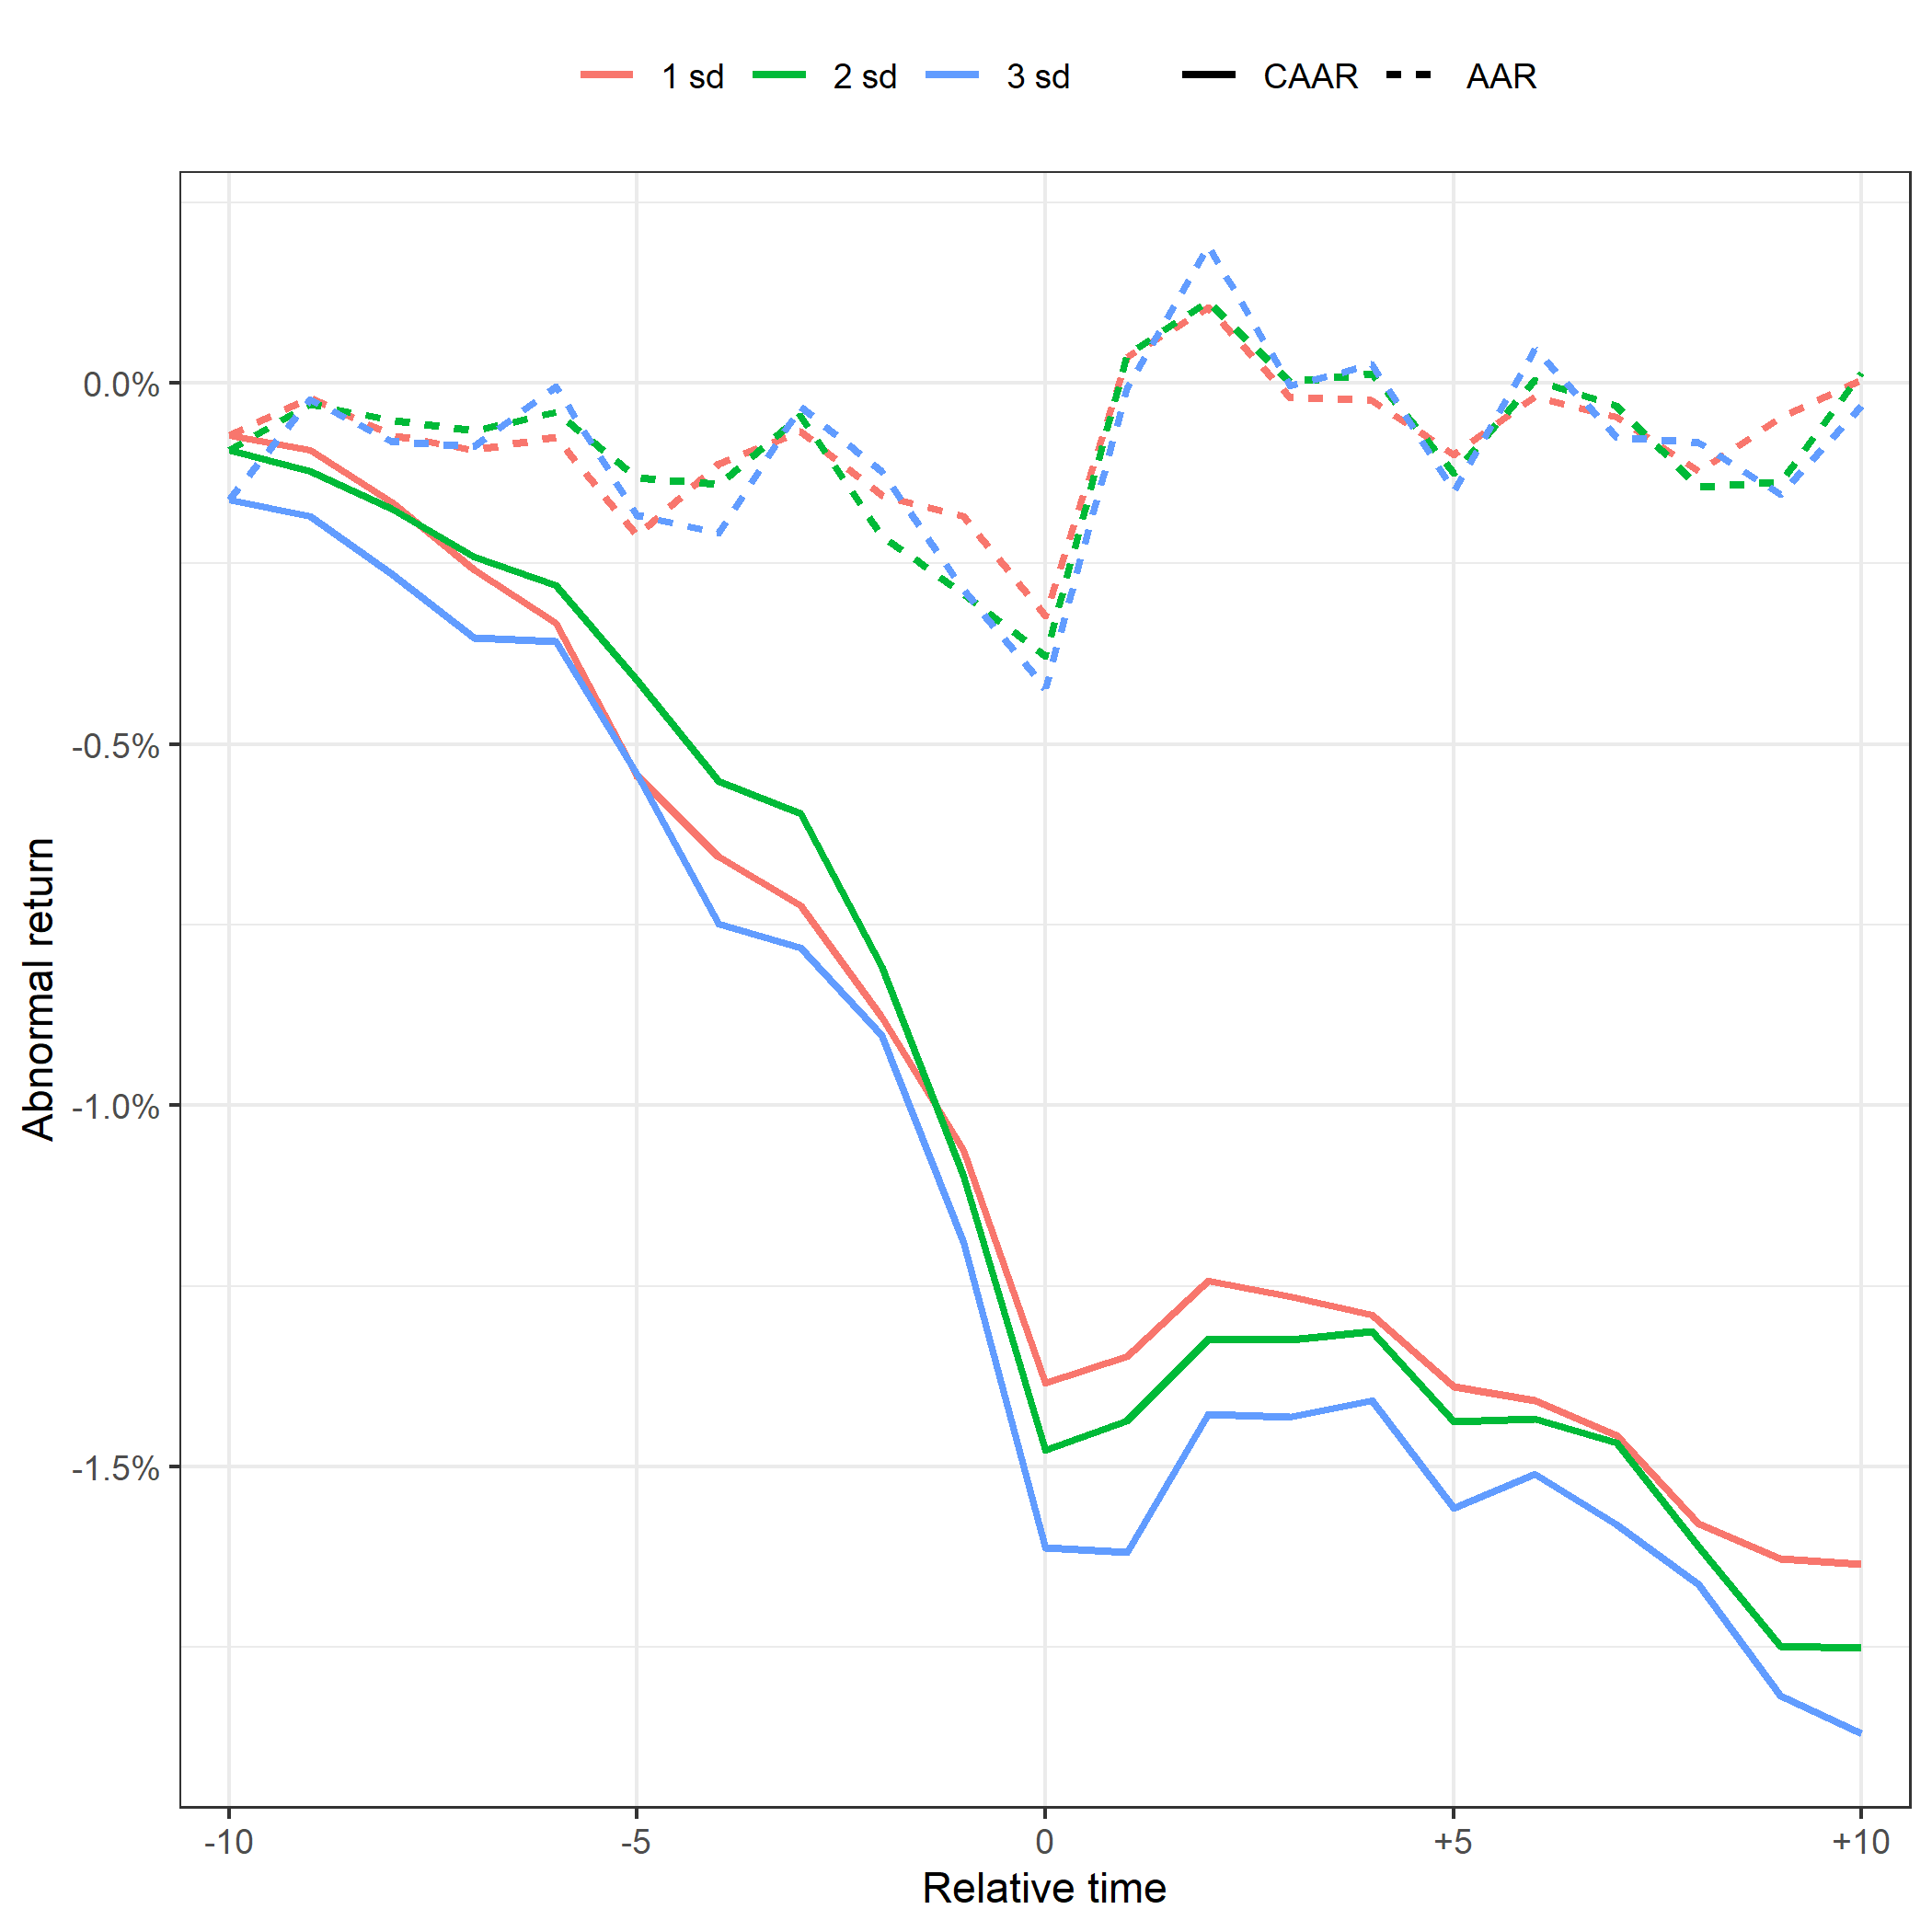
\includegraphics[scale=0.6]{Projekt/1.Figures analysis/ST_negative_sensitivity.png}
     \caption*{\footnotesize The figure illustrates the AAR and CAAR around the event date (t = 0) of negative news. The various colors represent the event identification rule of 1, 2, or 3 standard errors. The groups have, respectively, 1618, 957, and 683 events for 1,2, and 3 standard deviations}
    \label{fig:ST_neg_sensitivity}
\end{figure} 

The two new models, based on negative events, are compared to the original outcome (1sd) in figure \ref{fig:ST_neg_sensitivity}. The AAR is presented in dotted lines and the CAAR in solid lines for thresholds applying 2 sd (green) and 3 sd (blue). For simplicity, I have skipped the confidence intervals along with the bars. The similarities of the AAR and CAAR imply that the results are robust to changes in the event specification. Enforcing a stronger sd requirement leads to greater instantaneous impact on AAR on the event date. Moreover, a slight increase in CAAR signify a more severe reaction over the full window. 

\subsection{Market model: value vs. equal weights} \label{sec: sens_st_weights}

A portfolio of stocks needs to incorporate a weighted procedure in order to determine the relative impact the individual constituents should on portfolio performance. Figure \ref{fig:ST_neg_sensitivity_weight} compares the performance of applying value and equal weights to the an identical sample of firms experiencing negative events. 

\begin{figure}[H]
    \centering
    \caption{Negative news: Value vs. Equal weights}
    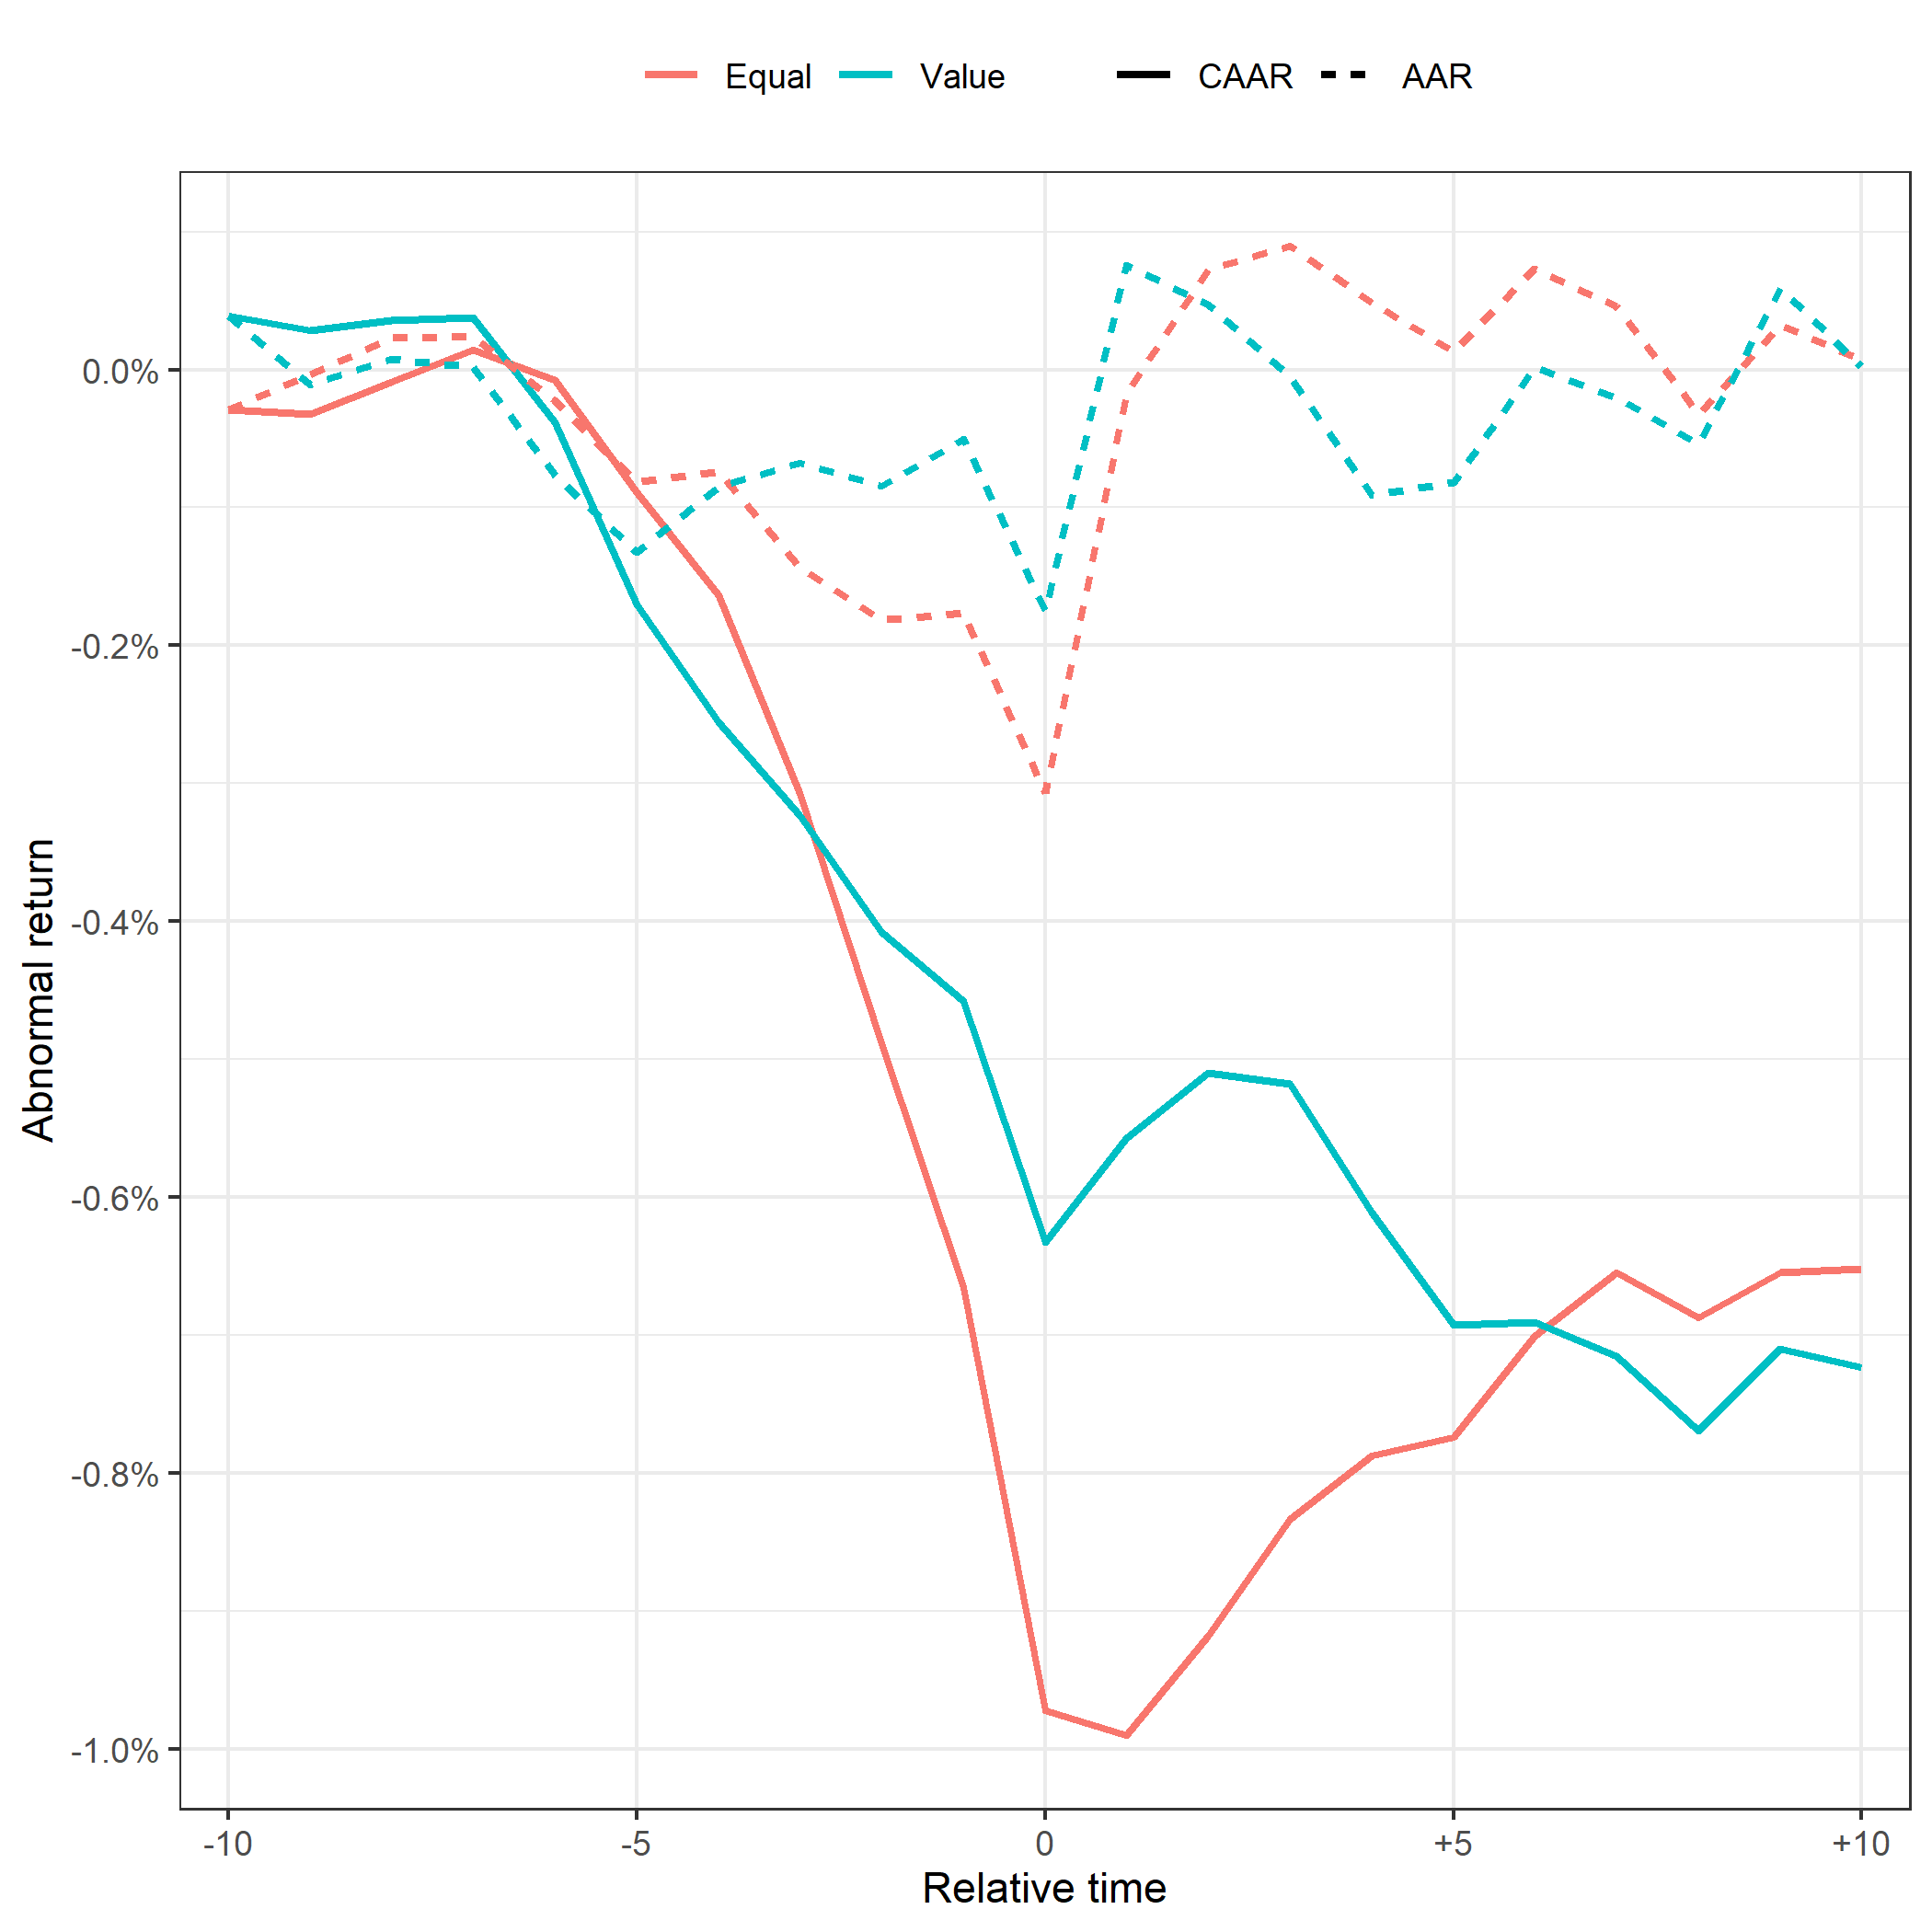
\includegraphics[scale=0.6]{Projekt/1.Figures analysis/ST_negative_sensitivity_weight.png}
     \caption*{\footnotesize The figure illustrates the average abnormal return (AAR) and cumulative AAR (CAAR) around the event date (t = 0) of negative news. The blue lines are returns calculated from an equally weighted portfolio, while the red lines are based on market capitalization weights.}
    \label{fig:ST_neg_sensitivity_weight}
\end{figure} 


The equal weighted portfolio returns validate the ordinary results, as the CAAR only diverge slightly and appear significant on the equal levels. While the portfolio AARs apparently follow each other to some extent, the development in CAAR is more adverse using equal weights relative to value weights. Applying equal weights inevitably allocates more weight to smaller stocks, which apparently contribute to less severe investor reactions. After the event has occurred the portfolio CAARs diverge, however as the AAR is statistically indifferent to zero in all days, the reactions are simply assumed to be minor estimation errors.    

\subsection{Calendar Time Portfolio: Portfolio weights}

Table \ref{tab: FF5_sensitivity} reports the alphas, t-values and significance levels of equally weighted portfolios along with the results from changing the threshold requirements. Besides the weights, the portfolio construction is identical to that from the empirical results in section \ref{sec: long_term_portfolio}. 

Altering the portfolio weights from value to equal clearly indicate a discrepancy from measurement with the latter generating higher absolute alpha values. The value weighted portfolio with T = 1 generated abnormal returns of -0.84\%, while the equivalent portfolio with equal weights ends up at -0.96\% significant on the $1\%$ level.   

The results are in contrast with the short term sensitivity analysis on portfolio weights, where the equal weighted portfolio generated lower abnormal returns. Again, the increased allocation toward smaller stocks seems to have an influential impact on the long run, however in the opposite direction relative to the short term. Applying holding periods of T = 8 and 12 months generate significant alpha as well indicating that smaller stocks are penalized over a longer time horizon than relatively larger ones.   

The abnormal returns of the equal weighted portfolios confirm the negative association between negative events and abnormal returns and to some degree the magnitude of the value weighted portfolio returns.

\setlength{\tabcolsep}{15pt}
\begin{table}[H]
\small
\centering
\caption{FF-5 alpha with equal weights and edit event rule } 
\makebox[\textwidth][c] {
\begin{tabular}{ccccccc}
\hline \hline \\ 
& &  Equal & & \multicolumn{2}{c}{ Value  } & \\ \cline{3-3} \cline{5-6}
  & & (1 SD) & & 2 SD  &  3 SD  & \\   
 & & & T = 1  & & \\ \cline{2-6}
 &  Alpha & $-0.96^{***}$  & &  -0.47  & -0.78  &  \\ 
 & t-value &  -3.80 &  & -0.97  & -1.63 & \\
 & &   & T = 4  & \\ \cline{2-6}
 & Alpha & $-0.70^{***}$ &  & $-0.45$ &  -0.27 & \\
 & t-value & -3.93 & & -1.58  & -1.04  & \\
 & &  & T = 8  & \\ \cline{2-6}
 & Alpha  & $-0.64^{***}$ & & -0.14 & -0.12 &  \\
 & t-value  & -4.20 & & -0.89 & -0.68 & \\
& &  & T = 12  & \\ \cline{2-6}
 & Alpha  & $-0.49^{***}$ &  & -0.16 & -0.17 &  \\
 & t-value & -3.71 & & -1.16 &  -0.97  & \\ \hline \hline
 \multicolumn{7}{l}{ \footnotesize $^* \; p\; <\; 0.1$, $ ^{**} \; p\; <\; 0.05$, $ ^{***} \; p\; <\; 0.01$  } \\
 \multicolumn{7}{p{12cm}}{ \footnotesize Alpha is the WLS-regression intercept (in \%) of the Fama-French 5-factor model, displayed along with the corresponding t-value. N is the average amount of firms included in the portfolio each month, and T is the portfolio holding period. The threshold for event firms to be included in the portfolio is either 1,2 or 3 "SD" (standard deviations) larger than the mean.} \\ 
 \hline
\end{tabular}
}
\label{tab: FF5_sensitivity}
\end{table}

\subsection{Calendar Time Portfolio: Thresholds}

Altering the threshold requirements from one to two and three standard leads to varying outcomes. For holding periods of one month, the alphas decrease and become insignificant from tightening the threshold, however the portfolio with three standard errors produce larger alphas than the one with two. With T = 4 the relation is reverse as the 2 standard deviation portfolio generates the largest alpha. Longer holding periods generate roughly equal abnormal returns across threshold values. As the portfolios are generating seemingly random outcomes, I reason that there is no relation between the event threshold and portfolio return on the long horizon. 


\subsection{New data}

\begin{figure}[H]
    \centering
    \caption{Negative news: Nasdaq Global}
    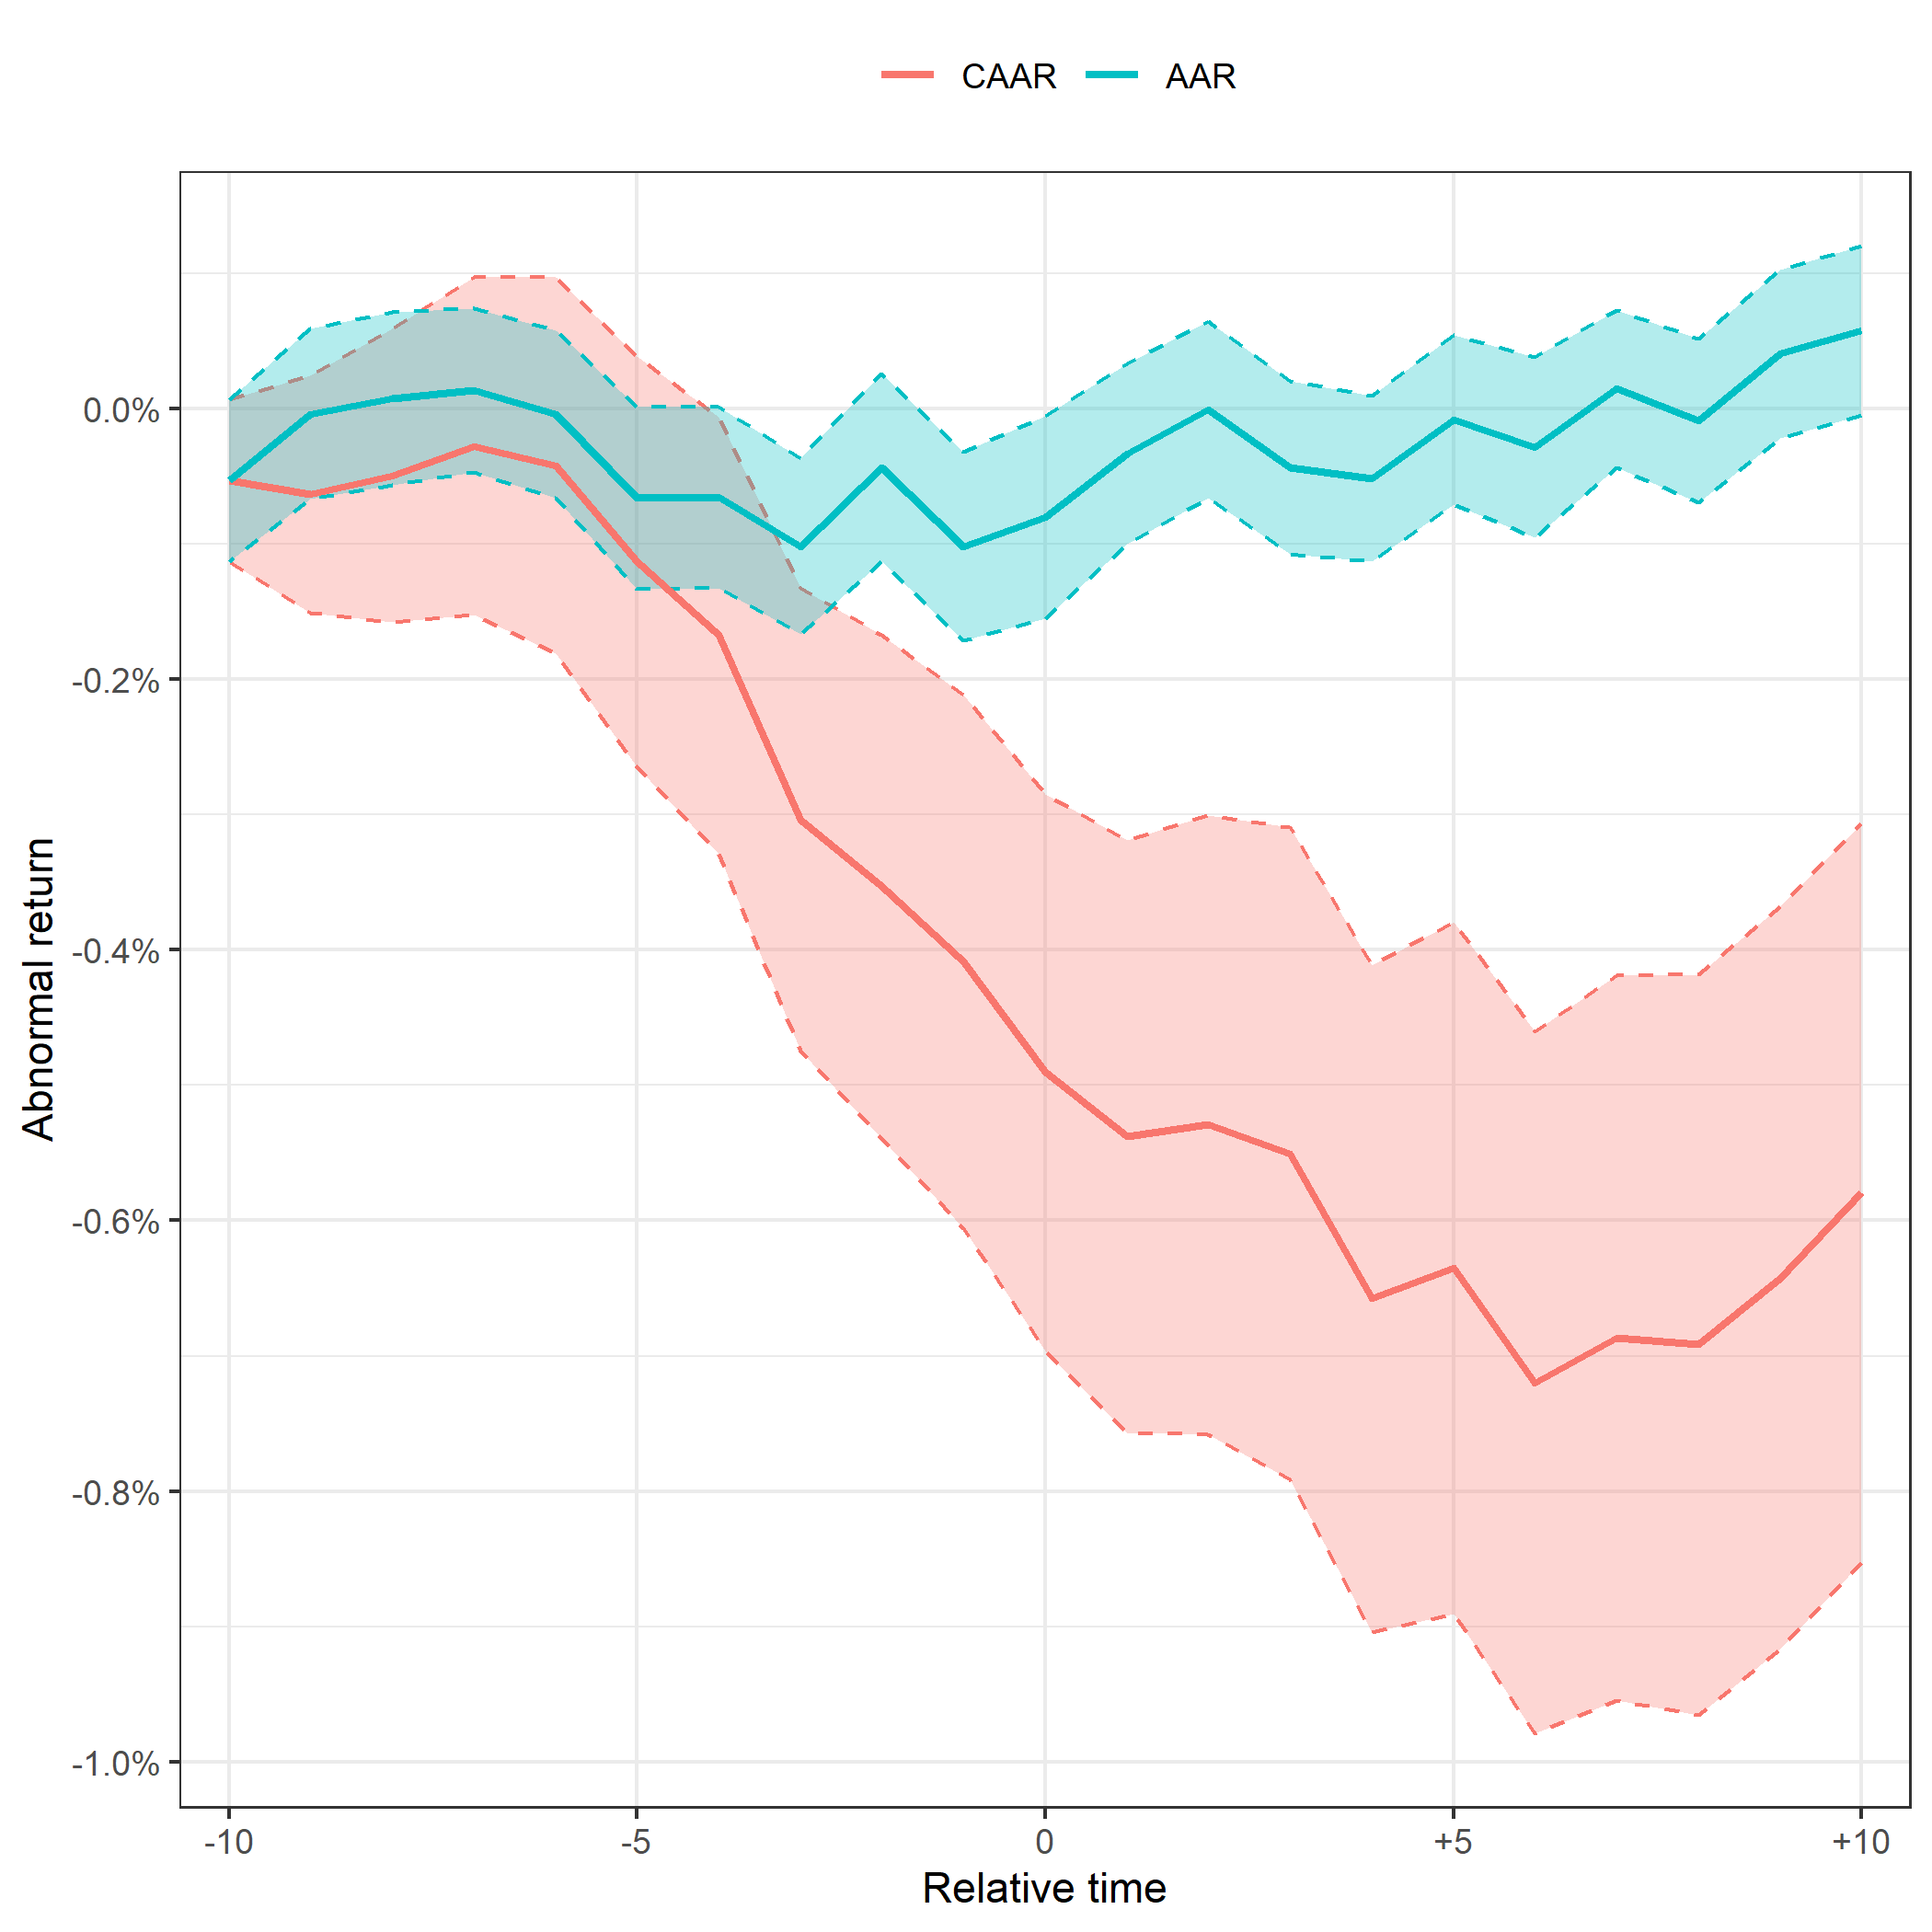
\includegraphics[scale=0.6]{Projekt/1.Figures analysis/ST_negative_all_CI_nasdaq.png}
     \caption*{\footnotesize The figure illustrates the average abnormal return (AAR) and cumulative AAR (CAAR) around the event date (t = 0) of negative news. The blue lines are returns calculated from an equally weighted portfolio, while the red lines are based on market capitalization weights.}
    \label{fig:ST_neg_sensitivity_weight}
\end{figure} 


\section{Analysis} \label{results}

The analysis is divided into three sections. First, in section \ref{sec: short_term_analysis} I focus on answering the hypotheses on short- and long-term performance from events related to the overall Social Development Goals, and to demonstrate the benefits of the sensitivity analysis. Then, the analysis shifts its focus towards building intuition and understanding regarding the sub-questions. In section \ref{sec: short_term_analysis_SDG}, I aim to determine whether investors place varying emphasis on different themes within sustainability. Finally, section \ref{ESG_reputation} delves into the relevance of firms' ESG risk characteristics when investors react to events.

\subsection{The impact of general SDG news on stock prices} \label{sec: short_term_analysis}
 
To answer the hypotheses, I assess the statistical significance and the intuition from the short- and long term results.  

\subsubsection{Short term hypothesis} 

The null hypothesis assumes that there is no market does reactions to news related to the SDGs within a short horizon. Any significant deviation from the expected returns suggest that sustainability-related news has notable influence on firm's market values.  \\
The significance of the results obtained from the Market Model is evaluated using a z-test. This test statistic is computed and compared to its assumed distribution under the null hypothesis that the abnormal returns are zero. The z-scores and corresponding significance levels, complementary to AAR on $t=0$ and CAAR 10 and 21 days surrounding the event, are presented in table \ref{tab: ST_neg_significance} for negative events and table \ref{tab: ST_pos_significance} for positive ones. The values presented in the tables are equivalent to the graphics in figures \ref{fig:ST_neg_news} and \ref{fig:ST_pos_news}. 

According to table \ref{tab: ST_neg_significance} negative SDG disclosures impact firms' market values significantly adverse not only on the event date but also over a 10-day and 21-day event window. In support of hypothesis 1.a the cumulative abnormal return is $-0.72\%$ throughout the 21-day event window. The observed impact of negative events is substantial and significantly below zero at the 1\% level of significance. As a result, I reject the hypothesis of no abnormal returns from negative events, and accept the alternative that negative events are associated with negative abnormal returns on average. 

Regarding positive news, the cumulative abnormal average change in market value around a 10- and 21-day event window is slightly negative. However, the results are insignificant, as indicated by the "Overall" column in table \ref{tab: ST_pos_significance}. With a CAAR of -0.02\% over the entire window, there is insufficient evidence to reject the null hypothesis. Hence, positive news related to the SDGs does not have a short term impact on firm's market values. Nonetheless, the AAR is significantly positive at the 1\% level with a value of 0.05\% on the event day. This suggest that a spike in positive news is instantly rewarded with a small increase in market value. However, this reaction alone is not sufficient to establish general intuition.

Accordingly, shareholders seem to penalize negative corporate social responsibility, while they do not really reward positive practices. 

\begin{table}[H]
\centering
\caption{Negative news: AAR and CAAR on overall and ESG risk level} 
\begin{tabular}{ccccc}
  \hline  \hline
  & \multicolumn{1}{c}{Overall} &  \multicolumn{1}{c}{Low} & \multicolumn{1}{c}{Medium} & \multicolumn{1}{c}{High}\\  
 \hline
$AAR_{t=0}$ &   $\underset{(-2.25)}{-0.17^{**}}$ &   $\underset{(-2.67)}{-0.22^{***}}$ &   $\underset{(-1.18)}{-0.13}$ &   $\underset{(-0.20}{-0.67 }$ \\

$CAAR_{[-5;+5]}$  &  $\underset{(-4.01)}{-0.65^{***}}$ &   $\underset{(-5.22)}{-1.39^{***}}$ &   $\underset{(-1.65)}{-0.36^{*}}$ &   $\underset{(-1.11)}{-0.52}$ \\ 

$CAAR_{[-10;+10]}$    & $\underset{(-3.21)}{-0.72^{***}}$ &   $\underset{(-4.49)}{-1.65^{***}}$ &   $\underset{(-1.80)}{-0.54^{**}}$ &   $\underset{(-0.38)}{-0.25}$ \\ 
   \hline \hline
   \multicolumn{5}{p{12cm}}{ \footnotesize $^* \; p\; <\; 0.1$, $ ^{**} \; p\; <\; 0.05$, $ ^{***} \; p\; <\; 0.01$  } \\
   \multicolumn{5}{p{13cm}}{\footnotesize The tables shows the CAAR and associated t-value related to positive and negative events over an event window of 10, and 21 days surrounding the event date along with the AAR on $t=0$. Negative events consists of 1046 observations. } \\
   \hline
\end{tabular}
\label{tab: ST_neg_significance}
\end{table}

The findings are in line with most of the previous literature. \cite{Blancard_ESG_sentiment} and \citep{kruger2015corporate} finds similar evidence of a short term pessimistic market reaction from negative news by applying the event study methodology and the Market Model as well. \citeauthor{Blancard_ESG_sentiment} identify slightly positive, but insignificant, abnormal return for positive events as well, whereas \citeauthor{kruger2015corporate} finds an ambivalent association that depends on the quality of the relation between the firms and their stakeholders. 

The short term shareholder reactions are in line with theories on efficient markets \citep{fama1969_EMH}, as the development in AAR is equivalent to shareholders promptly incorporate newly available information into to the market. While this is not a novel finding, the results of this paper provide evidence that shareholders do indeed integrate general information related to the Social Development Goals into their investment decisions. 

The Market Model appears to be a good choice for measuring abnormal returns in relation to negative news. In figure \ref{fig:ST_neg_news} the AAR is hovering around 0\% in the first four days of the window and again after the event has occurred at $t = 0$, implying that the expected returns are effective in reflecting the realized returns. The lack of a clear pattern in the reactions to positive news may be more indicative of the relative negligible impact of the news factor rather than criticism of the model.    

\begin{table}[H]
\centering
\caption{Positive news: AAR and CAAR (in \%) on overall and ESG risk level} 
\begin{tabular}{ccccc}
  \hline  \hline
  & \multicolumn{1}{c}{Overall} &  \multicolumn{1}{c}{Low} & \multicolumn{1}{c}{Medium} & \multicolumn{1}{c}{High}\\  
 \hline
$AAR_{t=0}$ &  $\underset{(3.22)}{0.05^{***}}$ & $\underset{(0.37)}{0.03}$ & $\underset{(1.05)}{0.08}$ &  $\underset{(0.20)}{0.16}$ \\ 
$CAAR_{[-5;+5]}$  & $\underset{(-1.18)}{-0.07}$ &  $\underset{(-0-55)}{-0.13 }$ &  $\underset{(0.22)}{0.05 }$ &  $\underset{(-0.91)}{-0.36}$ \\ 
$CAAR_{[-10;+10]}$    & $\underset{(-0.23)}{-0.02}$ &  $\underset{(-2.25)}{-0.23^{***}}$ &  $\underset{(1.86)}{0.24^{**}}$ &  $\underset{(-1.04)}{-0.34}$ \\ 
    \hline \hline
   \multicolumn{5}{p{12.5cm}}{ \footnotesize $^* \; p\; <\; 0.1$, $ ^{**} \; p\; <\; 0.05$, $ ^{***} \; p\; <\; 0.01$  } \\
   \multicolumn{5}{p{13cm}}{\footnotesize The tables shows the CAAR and associated t-value related to positive and negative events over an event window of 5, 10, and 21 days surrounding the event date along with the AAR on $t=0$. Positive and negative events consists of, respectively, 3564 and 1046 observations. } \\
   \hline
\end{tabular}
\label{tab: ST_pos_significance}
\end{table}

Likewise, the event study methodology works adequately at identifying negative events from spikes in news, as an evident investor reaction is recognized through the abnormal returns. However, the investor reaction materializes prior to the actual identification of events ($t=0$), which is a drawback of the event selection procedure. This issue arises since the underlying data set contains the frequency of firms being mentioned in news articles globally, rather than the precise timing of specific events. Consequently, the event identification procedure relies on detecting the largest events based on volume. As a results, the methodology may not fully capture the initial market response to "breaking" news, which is typically reflected in early investors reactions. These early reactions, characterized by significant drawdowns, are apparent in figure \ref{fig:ST_neg_news} between $t = -6$ and $t = 0$. \\
The incremental increases in the bars, from $t=-6$ preceding an event, indicates that, on average, the initial information regarding a particular event tends to be published approximately six business days prior to the event gaining significant attention from the outstanding media and experiences a spike in news coverage. During the period between $t=-6$ and $t=0$ investors gradually become aware of the event and react accordingly based on the information they acquire. 


\subsubsection{Long term hypothesis}

The hypotheses \#2 a and b aims to answer whether SDG-related news are associated with changes in firms' market values on long horizons. I assess the statistical significance of the alpha generated from portfolios that hold firms which have experienced a positive or negative event within T months. The regressions reveal significant monthly alphas of -0.84\% and -0.36\% from negative news portfolios with holding periods of one and four months, respectively. With these results I reject hypothesis 2.a, which implicate that negative news has a long term adverse impact, of at least four months, on the average firm's market value. The portfolios based on positive events do not generate significant alpha across any of the holding periods. Hence, I fail to reject the hypothesis that positive news related to the SDGs does not have a long term impact on market values.

However, the portfolio with a holding period of one month generates a negative alpha. This suggests that firms may be penalized when they are associated with positive interactions with the social development goals. Certain investors perceive interactions with SDGs and ESG as creating additional and unnecessary costs for the firm, which they believe may impact profitability negatively. For example, Fisher (2011) finds that companies making ESG-positive announcements are penalized by shareholders due to perceived conflicts with firm value maximization. 

\subsubsection{Threshold values}

The benefits from the sensitivity analysis are two-fold. First, the results validate the robustness of the initial findings. Second, it can broaden our knowledge on the drivers behind the results. 

Section \ref{sec: sens_st_sd} establish the impact of tightening the event threshold on the short-term abnormal returns. A more strict threshold directly affects which events get identified as important. Thus, the observed decrease in abnormal returns in figure \ref{fig:ST_neg_sensitivity} is not in line with expectations. There are no theoretical underpinnings of the result and it appears to be mostly an empirical issue in the sample. It appears that the events receiving the most public attention may not necessarily coincide with the events that investors value the most. 

The implications are similar for the long-term abnormal returns as demonstrated in table \ref{tab: FF5_sensitivity}. However, all the estimated alpha value becomes insignificant when tightening the threshold. 

On a side note, the monthly average amount of firms in the portfolios decrease by roughly half as the threshold is tightened by one standard deviation. For instance, with a holding period of one month, the portfolio with a threshold of one standard deviation consists of 18 firms on average, while tightening the threshold to two standard deviations reduces the number to 9. While the portfolios are sorted on negative events in order to capture the consequent factor, portfolios with fewer firms are inevitably exposed to higher levels of idiosyncratic risks arising from individual companies. Therefore, the likelihood, that the portfolio alpha is driven by specific company risks rather than a response to negative news, increases. The analysis conducted in this paper relies on diversification benefits achieved through rebalancing a random selection of stocks on a monthly basis. This approach allows to approximately isolate the effect of negative news on stock returns. Thus, reducing the number of firms, through e.g. tighter thresholds, has certain drawbacks, with one being that the portfolio returns may be exposed to unwanted factors besides that of the events. 


Anyway, based on the sign and magnitude of abnormal returns from the altered portfolio constructions, it appears that the original results accurately reflect the relation between negative events and investor reactions.  

\subsubsection{Changing portfolio weights}

Section \ref{sec: sens_st_weights} demonstrates that applying more relatively more weight to smaller firms, through an equal-weighted portfolio, increase the short-term abnormal returns through the period $t = -10$ to $t = 0$. On the one side, larger firms, on average, are anticipated to attract more media attention. Presumably, with greater news coverage, the stock price reaction is expected to be more severe due to 1) the news reach a larger potential investor base, and 2) investors receive comprehensive and more detailed information about the specific companies. On the other hand, the severe reaction among small stocks may be attributed to an overreaction when new information becomes available, which is plausible as the market value loss revert to approximately the level of the value weighted portfolio in the following days after more information becomes available. Anyhow, these explanations are not mutually exclusive. 

The findings from the long-term portfolios support this postulate, as relatively higher weight toward small stocks takes part in driving the alphas of the equal weighted portfolio lower for all holding periods.

A simple reason lies in the higher volatility of small stocks. The specific results from the short-term analysis are backed by the early research on media sentiment from \cite{tetlock_sentiment}. The author finds a larger price impact on small stocks relative to larger stocks from ordinary negative sentiment, due to their inherent larger volatility. Our methodologies are not alike, however. My analysis computes returns from companies based on the volume of firm-specific news, which may suppress small firms when applying value weights.  \citeauthor{tetlock_sentiment}, on the other hand, calculates the overall sentiment from a \textit{Wall Street Journal} column and measures the effect on a cross section of stocks, where volatility to general sentiment plays a large role for small stocks. 

The inherently higher volatility of small stocks play a similar role for equal weighted portfolio returns on the long run \citep{Fama_french_3fac}. 
Moreover, the discrepancy may be a feature of the Fama-French regressions. Tables \ref{tab: summary_neg_1} and \ref{tab: summary_neg_EW} in the appendix show the sensitivities to the risk factors of the value and equal weighted portfolios with a holding period of one month.  

Both portfolios have a positive beta to the market excess return in the range of 1.15-1.2 and to high-minus-low (value) of 0.31 and 0.22 for value and equal weights, respectively. With more allocation to smaller stocks, the equal weighted portfolio has a significant beta coefficient of 0.51 to the small-minus-big (size) factor. However, the value weighted portfolio has approximately zero sensitivity to the factor, with a value of -0.04. Although the r-squared is high at 0.89, it appears that the factor regression has issues with explaining the returns of the value weighted portfolios, with most of the variation in returns being explained by the market excess return and the value factor. The same issue does not pertain to the equal weighted portfolio, where the size factor explains a large part of the variations. 






\subsection{News impact from SDG Pillars} \label{sec: short_term_analysis_SDG}

The question in focus is whether specific dimensions of corporate social responsibility are more important to shareholders. The figures \ref{fig:ST_neg_bar} and \ref{fig:ST_pos_bar} illustrate that negative news concerning the SGD Pillars Prosperity, Peace, and Partnership leads to significantly pessimistic market reactions on average, whereas no Pillar for positive news is associated with significant abnormal returns. Given these initial results along with the predominant focus on negative events in existing research, this section will place greater emphasis on analyzing the impact of adverse news. 

Negative news related to Prosperity demonstrates a CAAR of -0.53\%, whereas positive news show no significant impact on returns with a value of approximately 0.1\%. The Prosperity Pillar is mostly driven by SDG 7 (Affordable and Clean Energy) and 8 (Decent work and Economic Growth) which account for 71\% of the volume in negative events. SDG 7 relates to the global transition to sustainable energy sources, in line with the objectives defined in the Paris Agreement, which describes climate risk as a systematic risk. While SDG 7 is associated with many events, the corresponding investor reaction remains close to zero both regarding positive and negative news. This suggests that while there is a significant public attention, these events may be perceived as relatively unimportant from a corporate perspective. However, \cite{hart1996does} finds a positive relation between reducing emissions and financial performance for a sample of S\&P 500 firms. A newer study from \cite{being_green} elaborates on the relation and shows that neither low-emission or high-emission companies with higher environmental scores perform better financially. According to the the article, companies that do not live up to environmental standards are not necessarily penalized from a profit-maximization perspective. On a side note, even though former research indicates that high-emission, or in other ways low ESG, companies are not penalized financially, they bear the risk of being black-listed by institutional investors with high ESG portfolio requirements, which as an isolated event is expected to increase divestments by other investors further \cite{dell2021norwegian}. 

The Peace Pillar encompass SDG 16 (Peace, Justice and Strong Institutions) solely. The keywords, peace and strong institutions, are not typically associated with important corporate events and financial performance. Justice, on the other hand, is crucial for both, as the keyword related to various negative corporate events like accounting fraud and market manipulation. Consequently, SDG 16 is linked to more than 1400 negative events, surpassing all other SDGs by a decent margin. Events tied to the SDG also exhibit a large and significant average drop in market value, with a CAAR of approximately -0.57\% throughout the entire window. A short term event study conducted by \cite{bauer2010misdeeds} examining alleged corporate misconduct involving governance-related offenses reveal that investors react negatively to corporate filings before any verdict is published. The study reports an average CAAR of -11.6\% based on a Fama-French 3 factors model over a 21-day window. Given the significant declines observed from actual filings, the investor reaction from spikes in news related to similar events seem appropriate. As mentioned in the literature review in section \ref{lit_rev}, the disparity in methodologies between identifying events based on media activity (as in this case) and hand-picking specific events, as done in \citeauthor{bauer2010misdeeds}) results in discrepancies in results - in this case an average difference of more than 11\%-points. 

The short term reaction to negative news concerning the Pillar, Planet, generates the highest abnormal return at -0.7\%. The overall theme incorporates development goals related to tangible subjects as climate action, responsible production, and the earth as a whole, which has received much public attention in the 21st century.

The Pillar "Planet" obtains the highest negative abnormal return of -0.7\% from negative events and a relatively high abnormal return of 0.1\% for positive events in the short term. This can be attributed to the pillar's focus on development goals related to tangible subjects such as climate action and responsible production. These issues have received significant public attention in the 21st century, possibly resulting in a heightened investor attention as well. Extensive research has been conducted in this area. For instance, \cite{karpoff2005reputational} find that the average legal penalty for environmental violations is around 2.26\%, and the market penalty is roughly of similar magnitude. Similarly, \cite{capelle2010does} discovers an average market penalty of -1.3\% in terms of market value from industrial disasters. Figure \ref{fig:event_distribution_SDG} shows that, within this theme, most of the identified events are related to responsible production (SDG 12) and climate action (SDG 13). Hence, the SDGs draw a lot of public attention, however investor are mostly reacting to the former when considering negative events. 

Among the Five Pillars, People and Partnership stands out with positive, although insignificant, CAAR values of 0.48\% and 0.37\%, respectively, concerning negative events.
The Partnership Pillar focuses solely on SDG 17 (Partnerships for the Goals). The SDG in itself is relatively vague and supposedly difficult to quantify, as the main message is to strengthen the implementation of global partnerships. The underlying catalyst for these events are driven by some firms falsely proclaiming to be sustainable across various aspects. Such strategies, commonly referred to as 'green-washing,' are heavily disapproved of by activist groups and also penalized in financial markets, if discovered. News concerning green-washing is related to SDG 17, which is expected to be the main driver of the abnormal returns. The average value of the abnormal returns across companies is positive, however the wide confidence bands indicate that it comes with high uncertainty. Thus, a large part of the reactions must be negative.  \cite{Blancard_ESG_sentiment} backs up the argument of investors punishing such misconduct, but also note that successful green-washing can help mitigate the financial penalties from adverse ESG events. Overall, the Partnership Pillar is associated with positive, but uncertain, average abnormal returns, but the negative parts of it is expected to be a result of revealed green-washing. 

The People Pillar, which encompasses development goals related to poverty reduction, quality education, gender equality, and more, presents challenges when it comes to quantifying social corporate behavior. As the SDGs within this pillar are more related to supporting developing countries, it is uncommon for regular firms to take a large part, which in part is reflected through the relatively low amount of events for these SDGs, as per figure \ref{fig:event_distribution_SDG}. Thus, immoral acts in this context may be better reflected through long term rather than short term investor reactions. For instance, SDG 3 (Good Health and Well Being) has the second highest number of negative and positive events among the SDGs, however the investor reaction is minimal. The volume of events indicates the media considers well-being of people as a important theme, but investors do not view it as essential from a corporate or profit-maximization perspective.   


Whether SDG news are important for shareholders is clearly dependent on which theme the news is related to. Negative news related to the Pillars Planet, Peace, and Prosperity generate negative abnormal returns at -0.70\%, -0.57\%, and -0.53, respectively, with the two former being significant at 5\%. On the other hand, People and Partnership generates positive abnormal returns of 0.48\% and 0.37\%, respectively. The characteristics of the former groups are more tangible than the latter, which in the end helps in generating more significant investor reactions. Overall, there is clear evidence that investors value certain characteristics within the Social Development Goals higher than others. 


\subsection{Impact of ESG risk reputation} \label{ESG_reputation}

Generalizing changes in stock returns to overall and specific SDG news provide a good empirical understanding of how investors integrate corporate sustainability in their decision making. However, companies are facing different issues and risks toward ESG, hence external investor pressure might vary accordingly. 
The literature on the effect of reputation is inconclusive. On the one hand, some argue that firms with a good reputation will face more severe investor reactions from failing to live up to their status. \cite{noNewsgoodnews} backs this claim from a media perspective, as they find that accidents related to companies with an admirable CSR record are far more likely to be reported in the media. Others, like \cite{flammer2013corporate} and \cite{godfrey2009relationship}, argue that a history of strong corporate responsibility will mitigate the social pressure from adverse events, meaning that firms with a good reputation experience less decrease of market value from negative ESG news. Moreover, \cite{Blancard_ESG_sentiment} point out that a firm's sector ESG reputation can mitigate the market value loss from negative events.  

Initially, we need to pay attention to the way ESG reputation is defined. \cite{rennings2007effect} point out that outcomes may differ depending on whether reputation is calculated relative to industry peers or not. The ESG Risk Ratings applied in this study are absolute, hence a rating is comparable across all sub-industries. 

The illustrations from figure \ref{fig:ST_neg_ESG} are in contrast with the latter theories. The results from the graph are concretized in table \ref{tab: ST_neg_significance} along with significance levels of 10 and 21 day CAAR. Firms with low ESG risk are penalized more heavily after negative events compared to medium and high-risk firms. As a natural virtue of the rating, firms with low ESG-risks comes with a premium, as they are expected to avoid extreme negative events related to corporate sustainability. For example, a low-risk company may have a relatively high market valuation based on their current status. If they disappoint on ESG-related topics, investors need to adjust their expectations about such events happening in the future and the corresponding change in market value they place with the firm's sustainability profile. The distinction between theory and results may appear due to the media effect as described by \cite{noNewsgoodnews}, with the argument that low-risk firms are more exposed to the media in case of negative events. With that being said, I cannot prove whether the distinctions in market reaction is a consequence of the samples and time periods applied. 

Firms with high ESG-risk are encountering no change in market value from negative news. If investors place a fairly high probability of negative events occurring for high-risk firms, then the risk of an actual events seems to be priced into the market value apriori. Medium ESG-risk firms are experiencing negative abnormal returns, however less negative than low-risk firms, which seems on par with an intermediate investor reaction.  

The reaction to positive news is less clear cut. Medium-risk firms experience abnormal returns from positive events, as expected, while low-risk firms bear market value losses. I find no theoretical underpinnings for the distinction in abnormal returns between the two groups in the literature. Although, \cite{flammer2013corporate} does report that positive market reactions to eco-friendly events are smaller for companies with low environmental risk, and that the increasing social pressure to become green has resulted in decreased reactions to eco-friendly initiatives over time. Moreover, \cite{fisher2011voluntary} finds that positive ESG announcements have been found to be followed by negative abnormal returns, since these decisions often appear to be in contrast to profit-maximization.  
In addition,\cite{serafeim2022stock} finds that consensus ESG ratings predict future ESG news. Hence, a positive rating means investors expect mostly positive news in the future. Such a results can help explain why shareholders are not rewarding low-risk companies that experience a positive event, whereas medium risk firms are rewarded. Likewise, as high risk companies are expected to endure negative situations, they are not penalized to the same degree.  


Overall, I find a clear distinction between ESG-risk levels of companies and their abnormal returns from negative news related to the SDGs. 

\textbf{Long term:}

The gap between low and medium risk profiles does not persist on the long horizon. According to figure \ref{tab:FF5_neg_ESG} these portfolios generate abnormal returns of -0.64\% and -0.61\%, respectively, with a holding period of one month. The outcomes are similar for longer holding periods. 
Although the portfolios generate approximately equivalent alphas, the portfolio characteristics are completely different according to their sensitivities to the five factors, as illustrated in tables \ref{tab: summary_neg_ESG_L} and \ref{tab: summary_neg_ESG_M} in the appendix. For example, the low-risk portfolio is negatively correlated with the size factors at -0.28, whereas the medium risk portfolio has a coefficient of 0.41. Hence, it appears that the loss in market value from negative events are similar across company characteristics and risk toward ESG on a longer horizon. The sensitivities are estimated from the portfolios with holding periods of one month, however they are mostly similar for longer periods, but these values are not reported. 

Furthermore, the pattern cannot be fully generalized to inferences on longer horizons, due to the complete turnaround of the sign on alphas on high risk firms. The high risk portfolio has imminent issues with idiosyncratic risks as it consists of only 81 events and holds only 18 distinct firms throughout the full period, which inevitably plays a sizeable factor in the remarkably negative and fluctuating alpha outcome. Ignoring the outcome of the high risk portfolio, the remaining results do to some degree indicate a pattern similar to that of the short term due negative abnormal returns.

However, as the low and medium risk portfolios generate negative alphas of approximately the same magnitude, the long term abnormal returns are assumed to be independent of the level of companies' ESG-risks. 


\textbf{A slight phrase pre-conclusion on the discoveries from the analysis.}








\section{Discussion} \label{sec:discussion}
- To be able to actually trade this idea, we need a way of finding the negative events before they happen. 

- Future work could try to use the SDG signals (negative and positive events) as an indication of whether a company is expected to be downgraded, which there is some clear benefits in trading. I.e. refer to some paperps about this. 


 \renewcommand{\bibsection}{\section{Bibliography}}
\bibliography{Output/Litteraturliste}

\pagebreak

\appendix
\rhead{University of Copenhagen}
\lhead{Bilag}
\rfoot{Side \thepage}


\section{Appendix} \label{sec:appendix}

\subsection{Empirical results}

\begin{figure} [H]
    \centering
    \caption{Negative news: AAR split on relation to SDGs}
    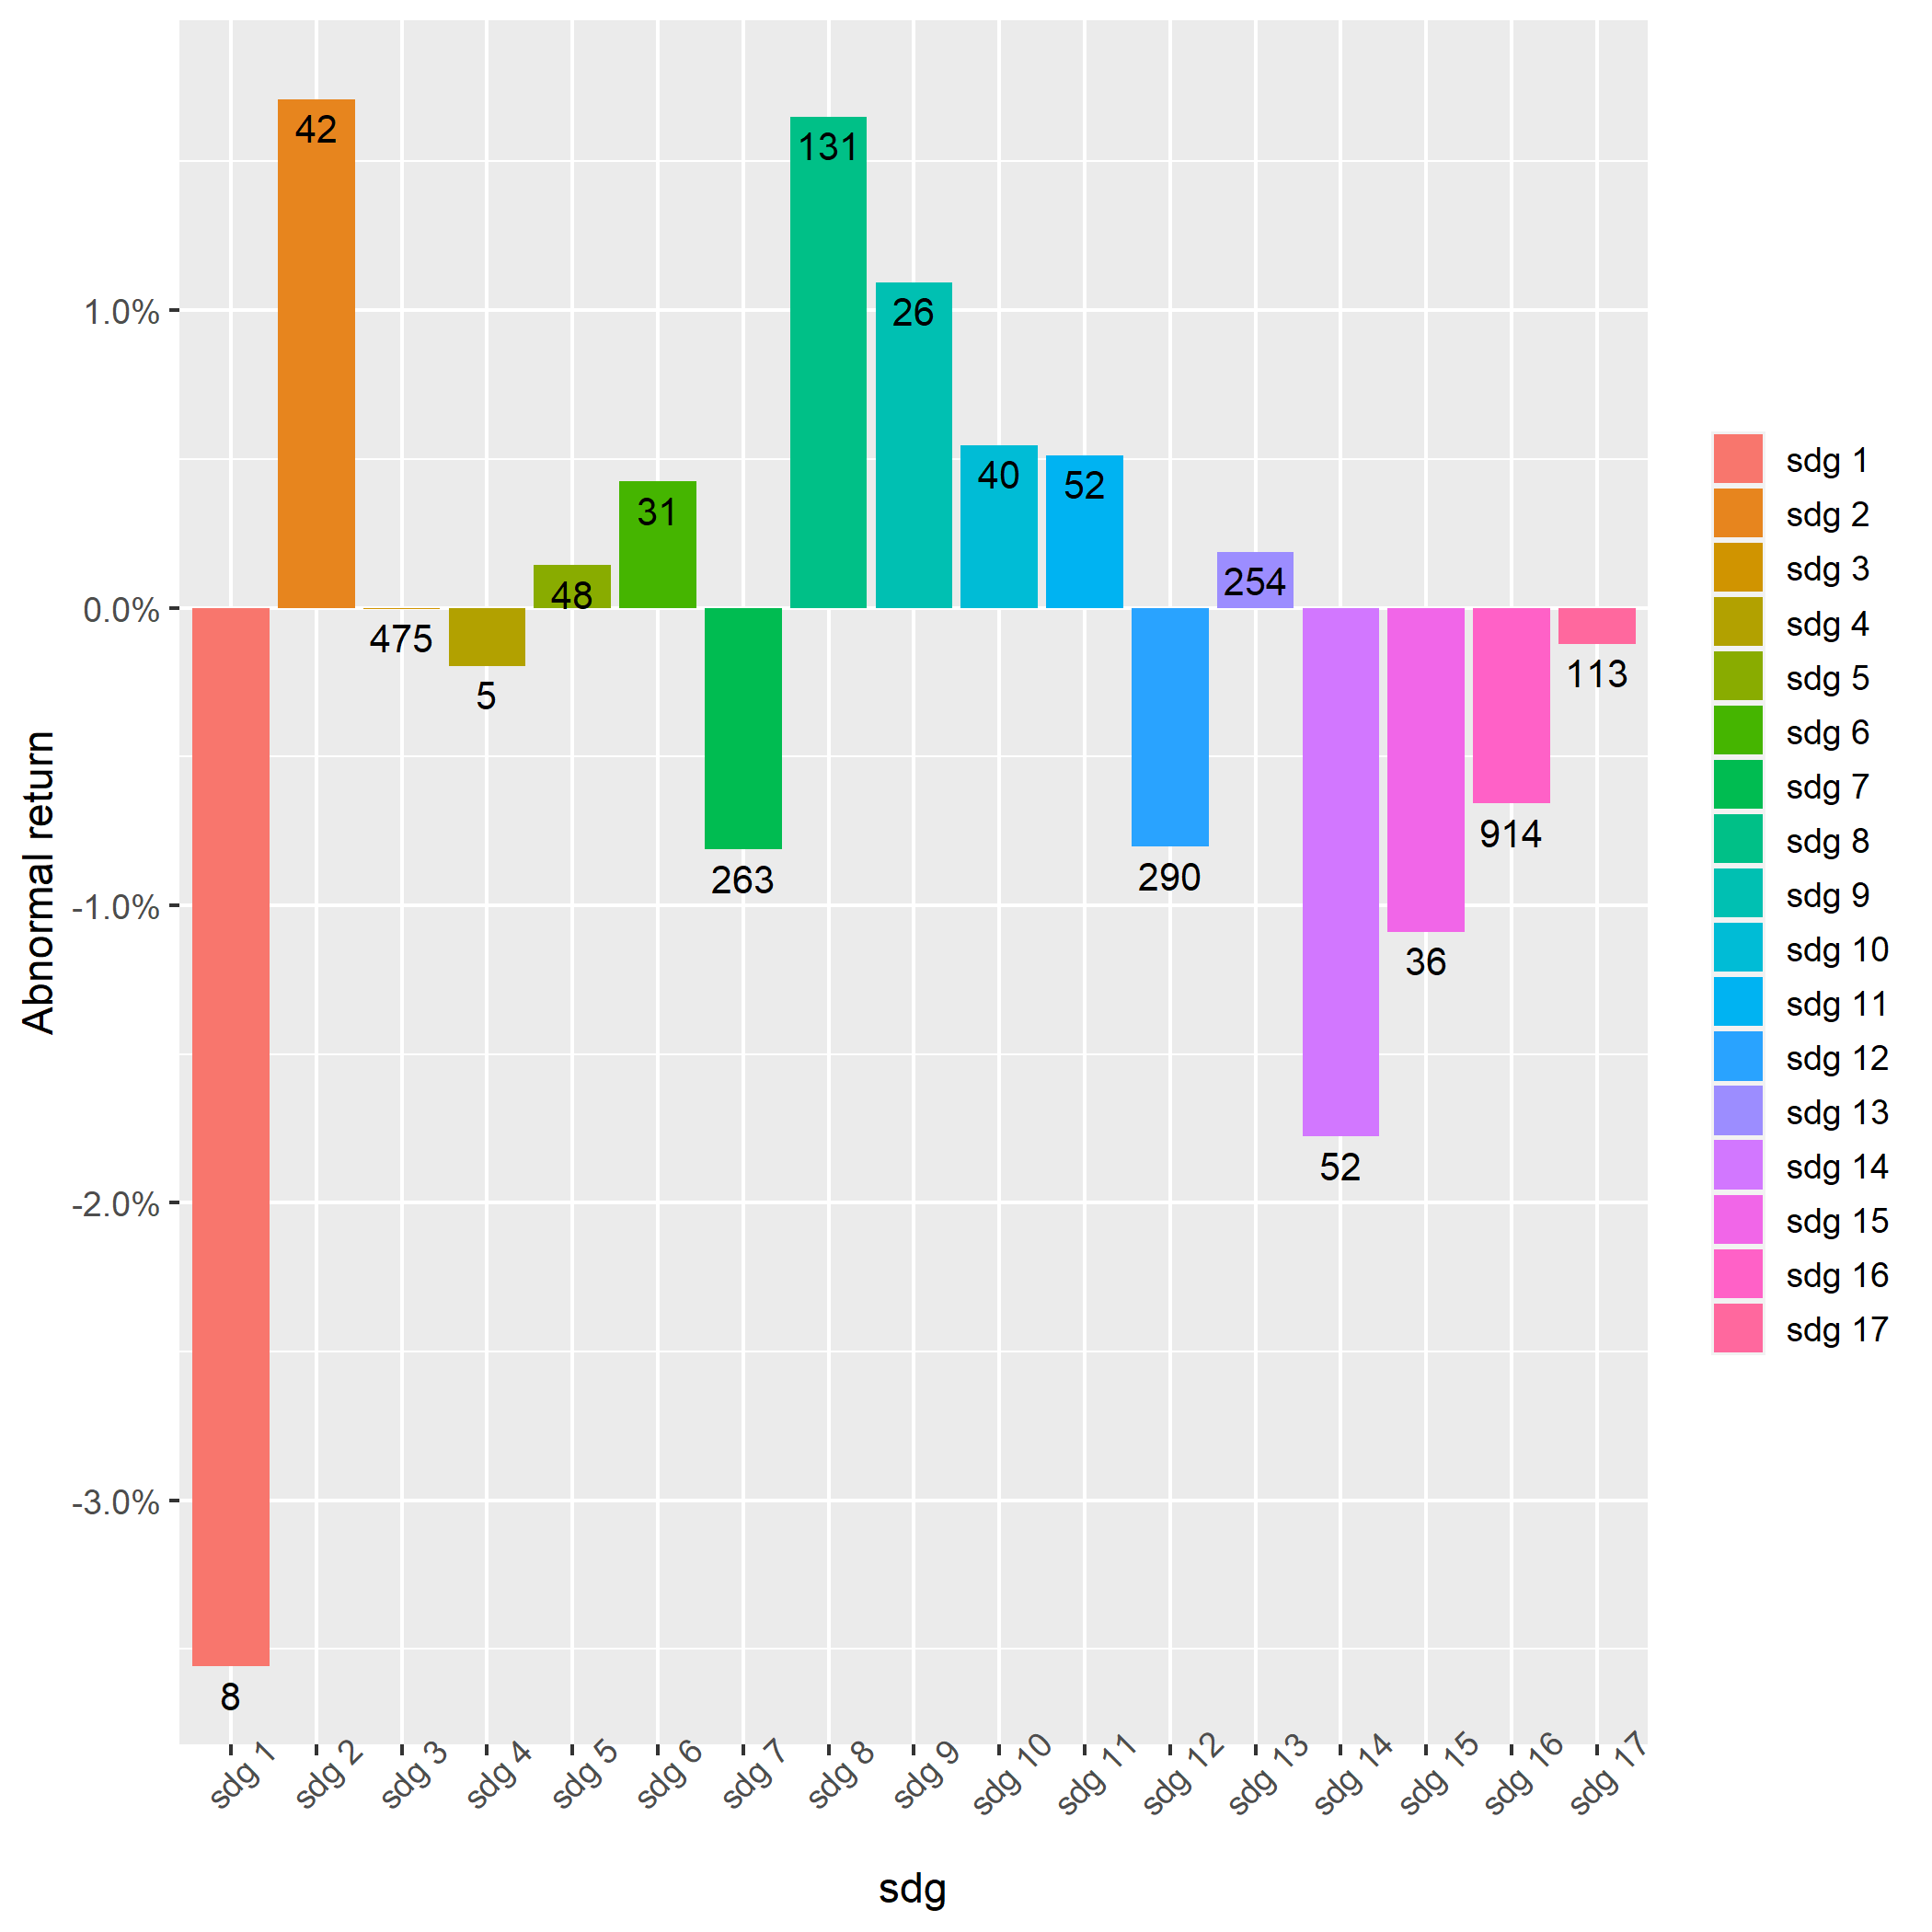
\includegraphics[scale=0.6]{Projekt/1.Figures analysis/ST_negative_sdg_bar.png}
    \caption*{\footnotesize The figure illustrates the AAR on $t = 0$ from negative news. The error bars represent the 95\% confidence intervals of the AAR.}
    \label{fig:ST_neg_bar_all}
\end{figure}

\begin{figure} [H]
    \centering
    \caption{AAR per SDG: positive news}
    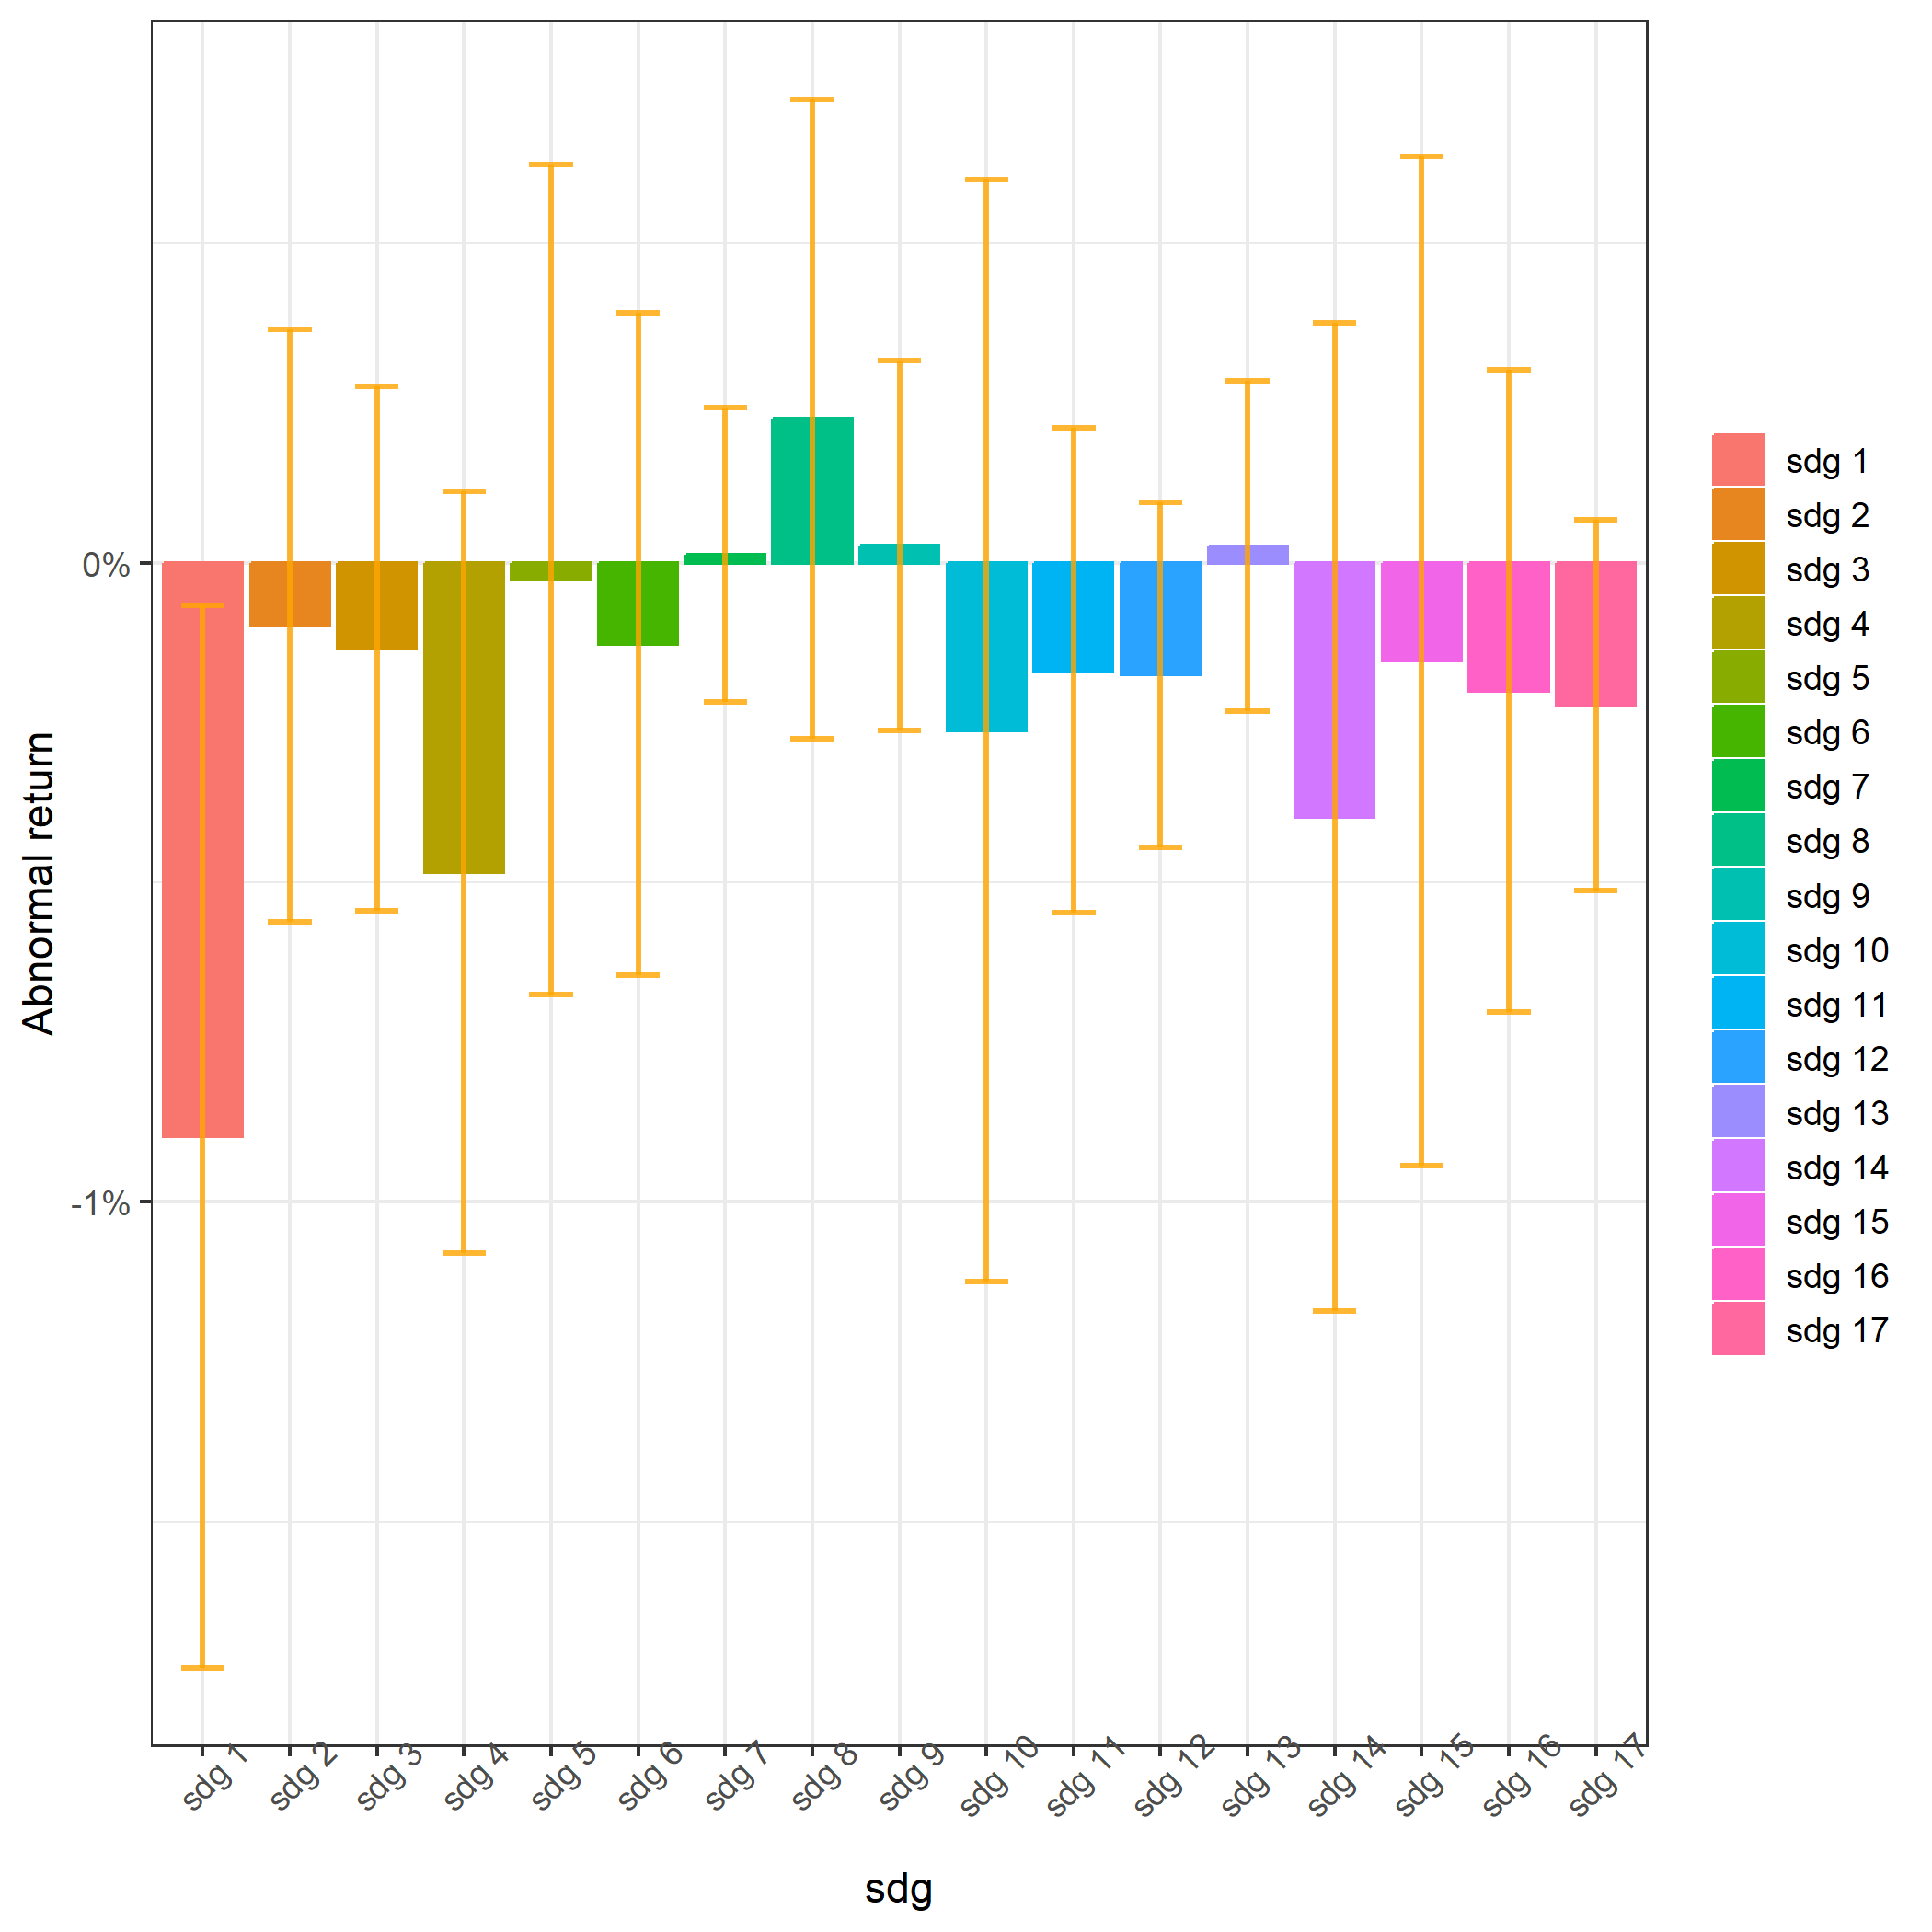
\includegraphics[scale=0.6]{Projekt/1.Figures analysis/ST_positive_sdg_bar.png}
    \caption*{\footnotesize The figure illustrates the AAR on $t = 0$ from positive news. The error bars represent the 95\% confidence intervals of the AAR.}
    \label{fig:ST_pos_bar_all}
\end{figure}




\subsection{Sensitivity analysis figures:}

\subsubsection{Short term}


\begin{table}[H]
\centering
\caption{AAR and CAAR (in \%) with new event rule (sd)} 
\begin{tabular}{lccccc}
  \hline  \hline
  & \multicolumn{2}{c}{Positive} &  & \multicolumn{2}{c}{Negative}\\ \cline{2-3} \cline{5-6}  
  & 2 sd & 3 sd & & 2 sd & 3 sd   \\   
 \hline
$AAR_{t=0}$ & $\underset{(0.875)}{0.051}$ & $\underset{(-0.278)}{-0.022}$ & & $\underset{(-3.409)}{-0.522^{***}}$ & $\underset{(-3.024)}{-0.617^{***}}$ \\ 
$CAAR_{[-2;+2]}$  & $\underset{(0.283)}{0.031}$  & $\underset{(0.631)}{0.089}$ & & $\underset{(-3.66)}{-0.714^{***}}$ & $\underset{(-2.648)}{-0.657^{***}}$ \\ 
$CAAR_{[-5;+5]}$  & $\underset{(1.197)}{0.195}$  & $\underset{(1.350)}{0.290}$ & &$\underset{(-3.56)}{-0.902^{***}}$ & $\underset{(-2.782)}{-0.867^{***}}$ \\ 
$CAAR_{[-10;+10]}$  & $\underset{(-0.168)}{-0.035}$  & $\underset{(-0.062)}{-0.018}$ &  & $\underset{(-1.886)}{-0.652^{*}}$ & $\underset{(-1.686)}{-0.697^{*}}$ \\ 
N & 1845 & 1078 & & 648 & 451  \\
   \hline \hline
   \multicolumn{6}{p{12cm}}{ \footnotesize $^* \; p\; <\; 0.1$, $ ^{**} \; p\; <\; 0.05$, $ ^{***} \; p\; <\; 0.01$  } \\
   \multicolumn{6}{p{13cm}}{\footnotesize The table shows the CAAR associated with positive and negative news over an event window of 5, 10, and 21 days surrounding the event date along with the AAR on $t=0$. The models are split on the requirement rule for included events (2 or 3 sd).} \\
   \hline
\end{tabular}
\label{tab:ST_sensitivity}
\end{table}


\begin{table}[H]
\centering
\caption{AAR and CAAR (in \%) with equally weighted returns} 
\begin{tabular}{lcccc}
  \hline  \hline
  & \multicolumn{1}{c}{Positive} &  \multicolumn{1}{c}{Negative}\\  
 \hline
$AAR_{t=0}$ &  $\underset{(0.634)}{0.045}$ & $\underset{(-3.509)}{-0.378^{***}}$ \\  
$CAAR_{[-5;+5]}$  & $\underset{(-1.233)}{-0.258}$ & $\underset{(-4.4255)}{-0.858^{***}}$ \\ 
$CAAR_{[-10;+10]}$    & $\underset{(-0.452)}{-0.128 }$ & $\underset{(-3.012)}{-0.822^{***}}$ \\ 
   \hline \hline
   \multicolumn{3}{p{10cm}}{ \footnotesize $^* \; p\; <\; 0.1$, $ ^{**} \; p\; <\; 0.05$, $ ^{***} \; p\; <\; 0.01$  } \\
   \multicolumn{3}{p{10cm}}{\footnotesize The tables shows the CAAR associated with positive and negative news over an event window of 5, 10, and 21 days surrounding the event date along with the AAR on $t=0$. The models are split on the requirement rule for included events (2 or 3 sd).} \\
   \hline
\end{tabular}
\label{tab:ST_sensitivity_weights}
\end{table}


\begin{figure} [H]
    \centering
    \caption{Positive news: event identification rule}
    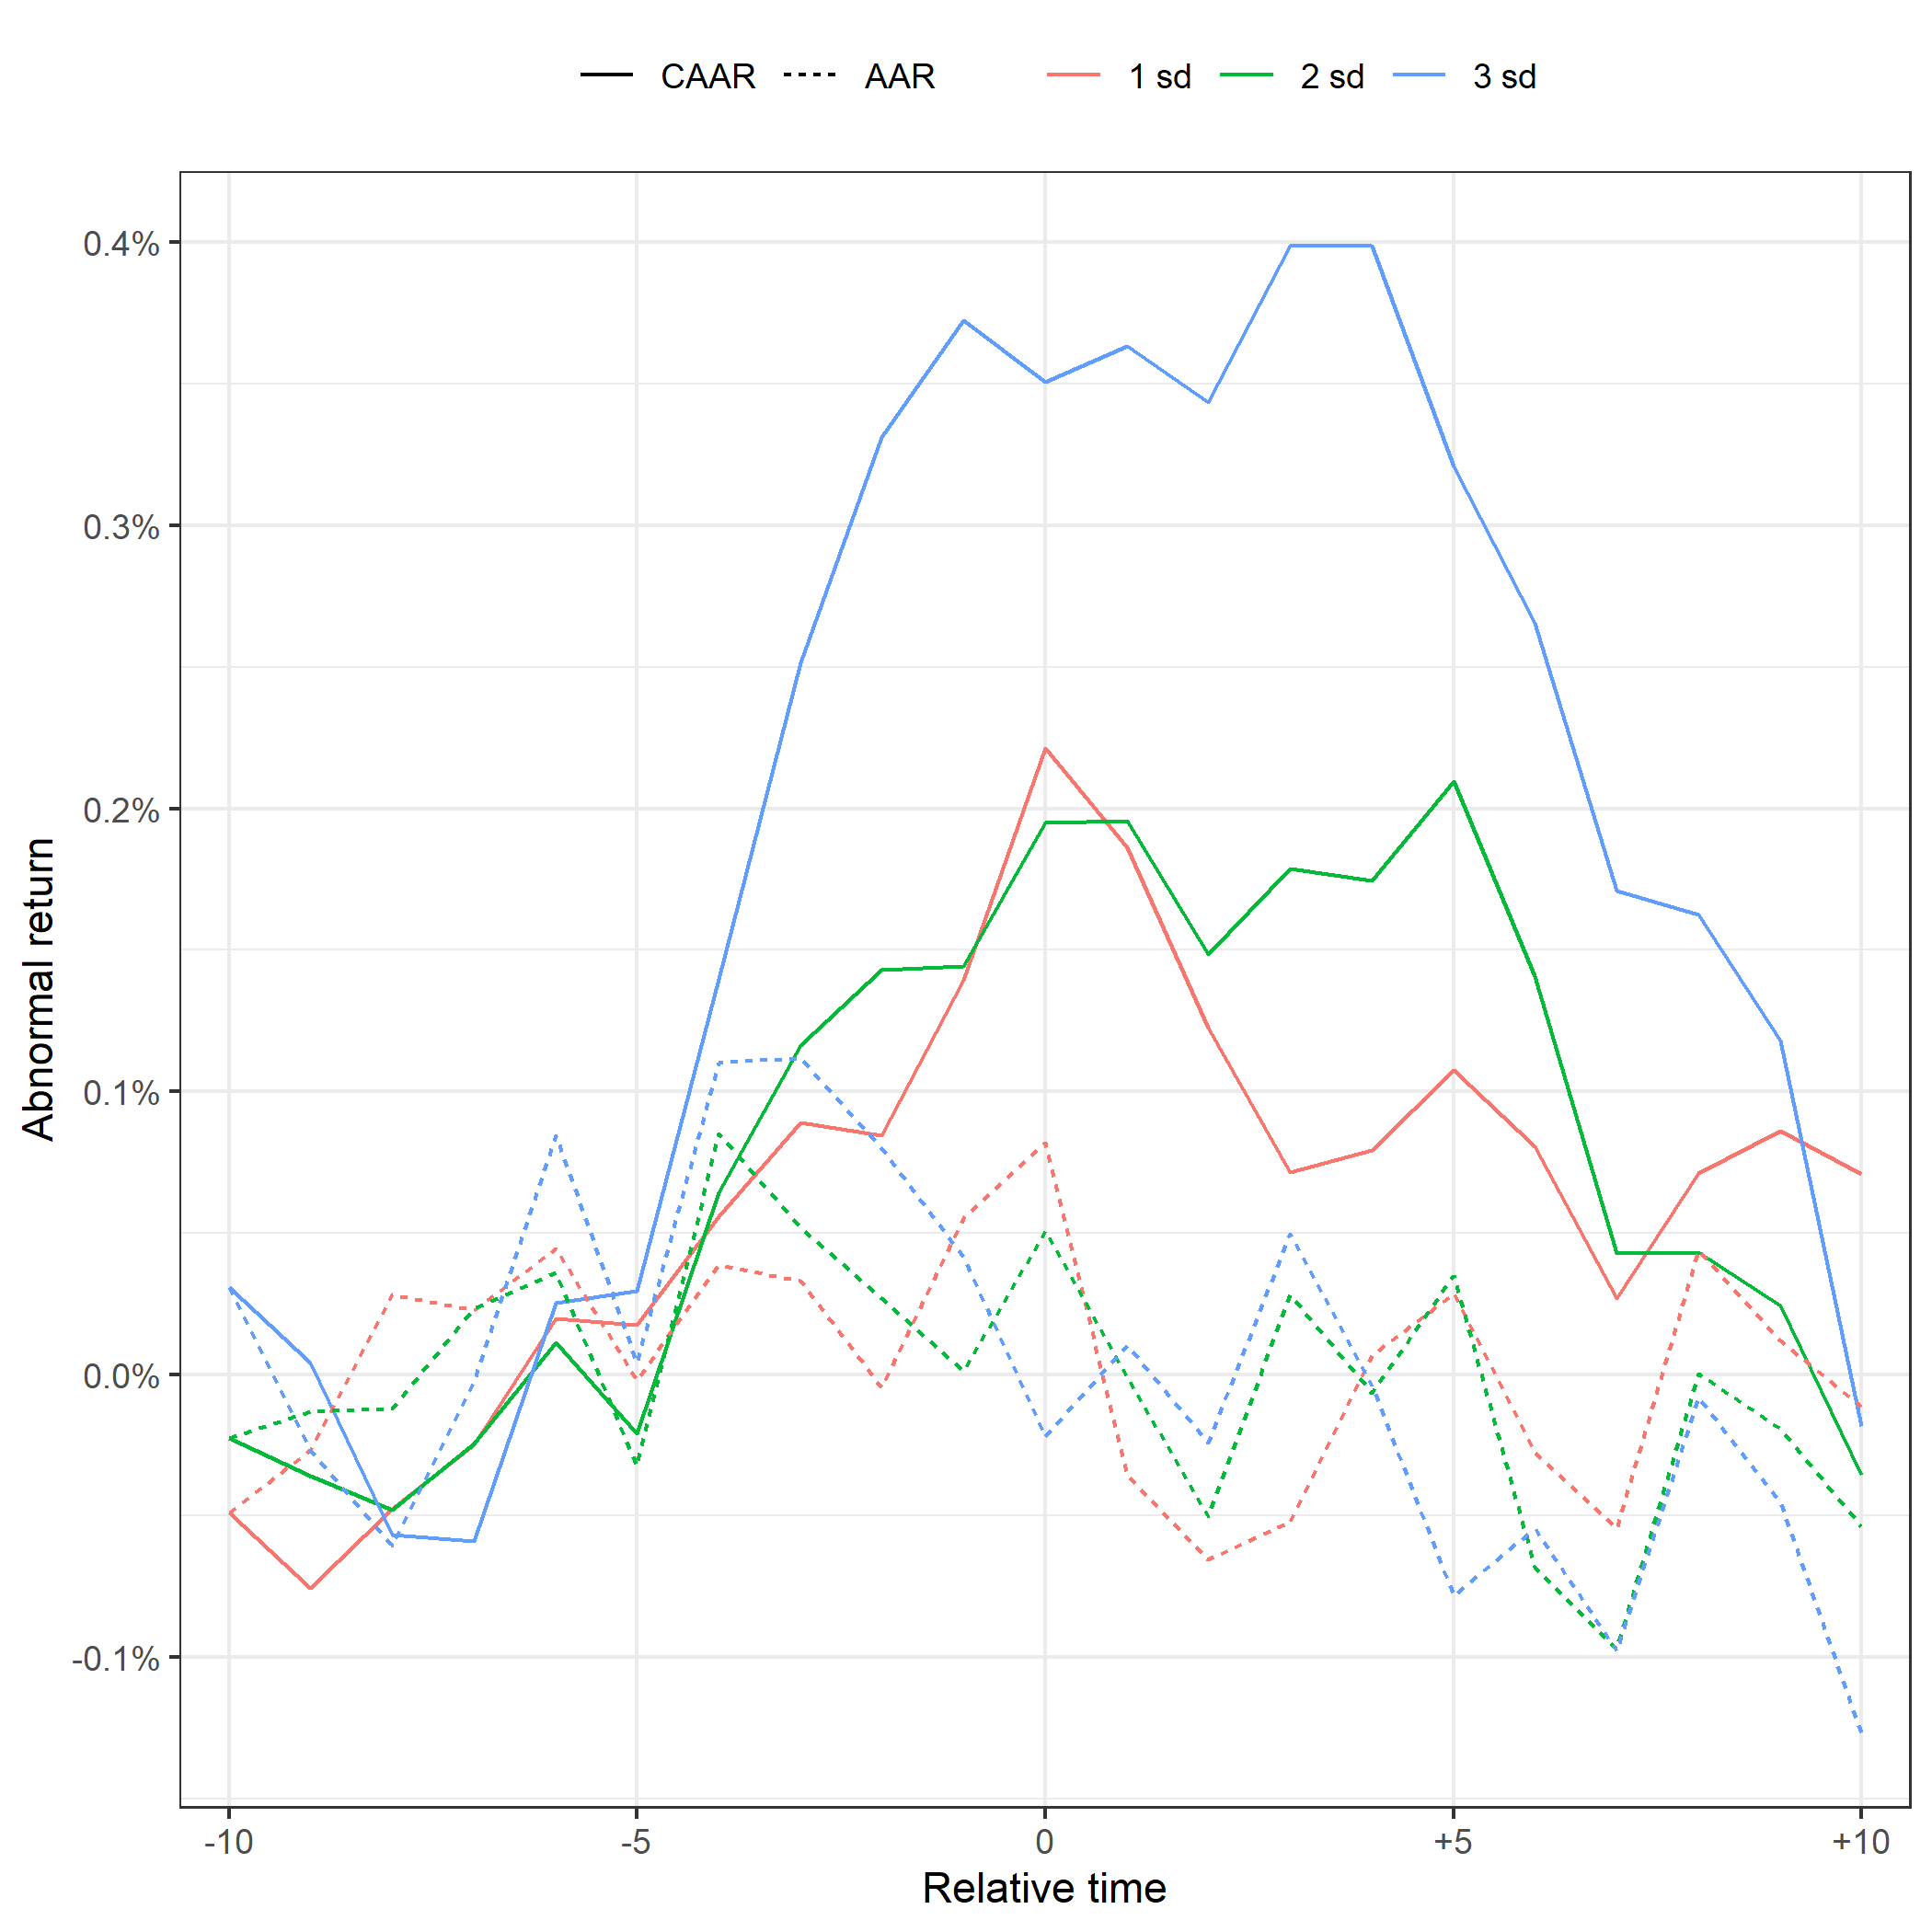
\includegraphics[scale=0.6]{Projekt/1.Figures analysis/ST_positive_sensitivity.png}
     \caption*{\footnotesize The figure illustrates the average abnormal return (AAR) and cumulative AAR (CAAR) around the event date (t = 0) of negative news. The figure illustrates the average abnormal return (AAR) and cumulative AAR (CAAR) around the event date (t = 0) of negative news. The various colors represent whether the event identification rule was based on 1, 2, or 3 standard errors. }
    \label{fig:ST_pos_sensi_sd}
\end{figure} 

\begin{figure} [H]
    \centering
    \caption{Positive news: Value vs. Equal weights}
    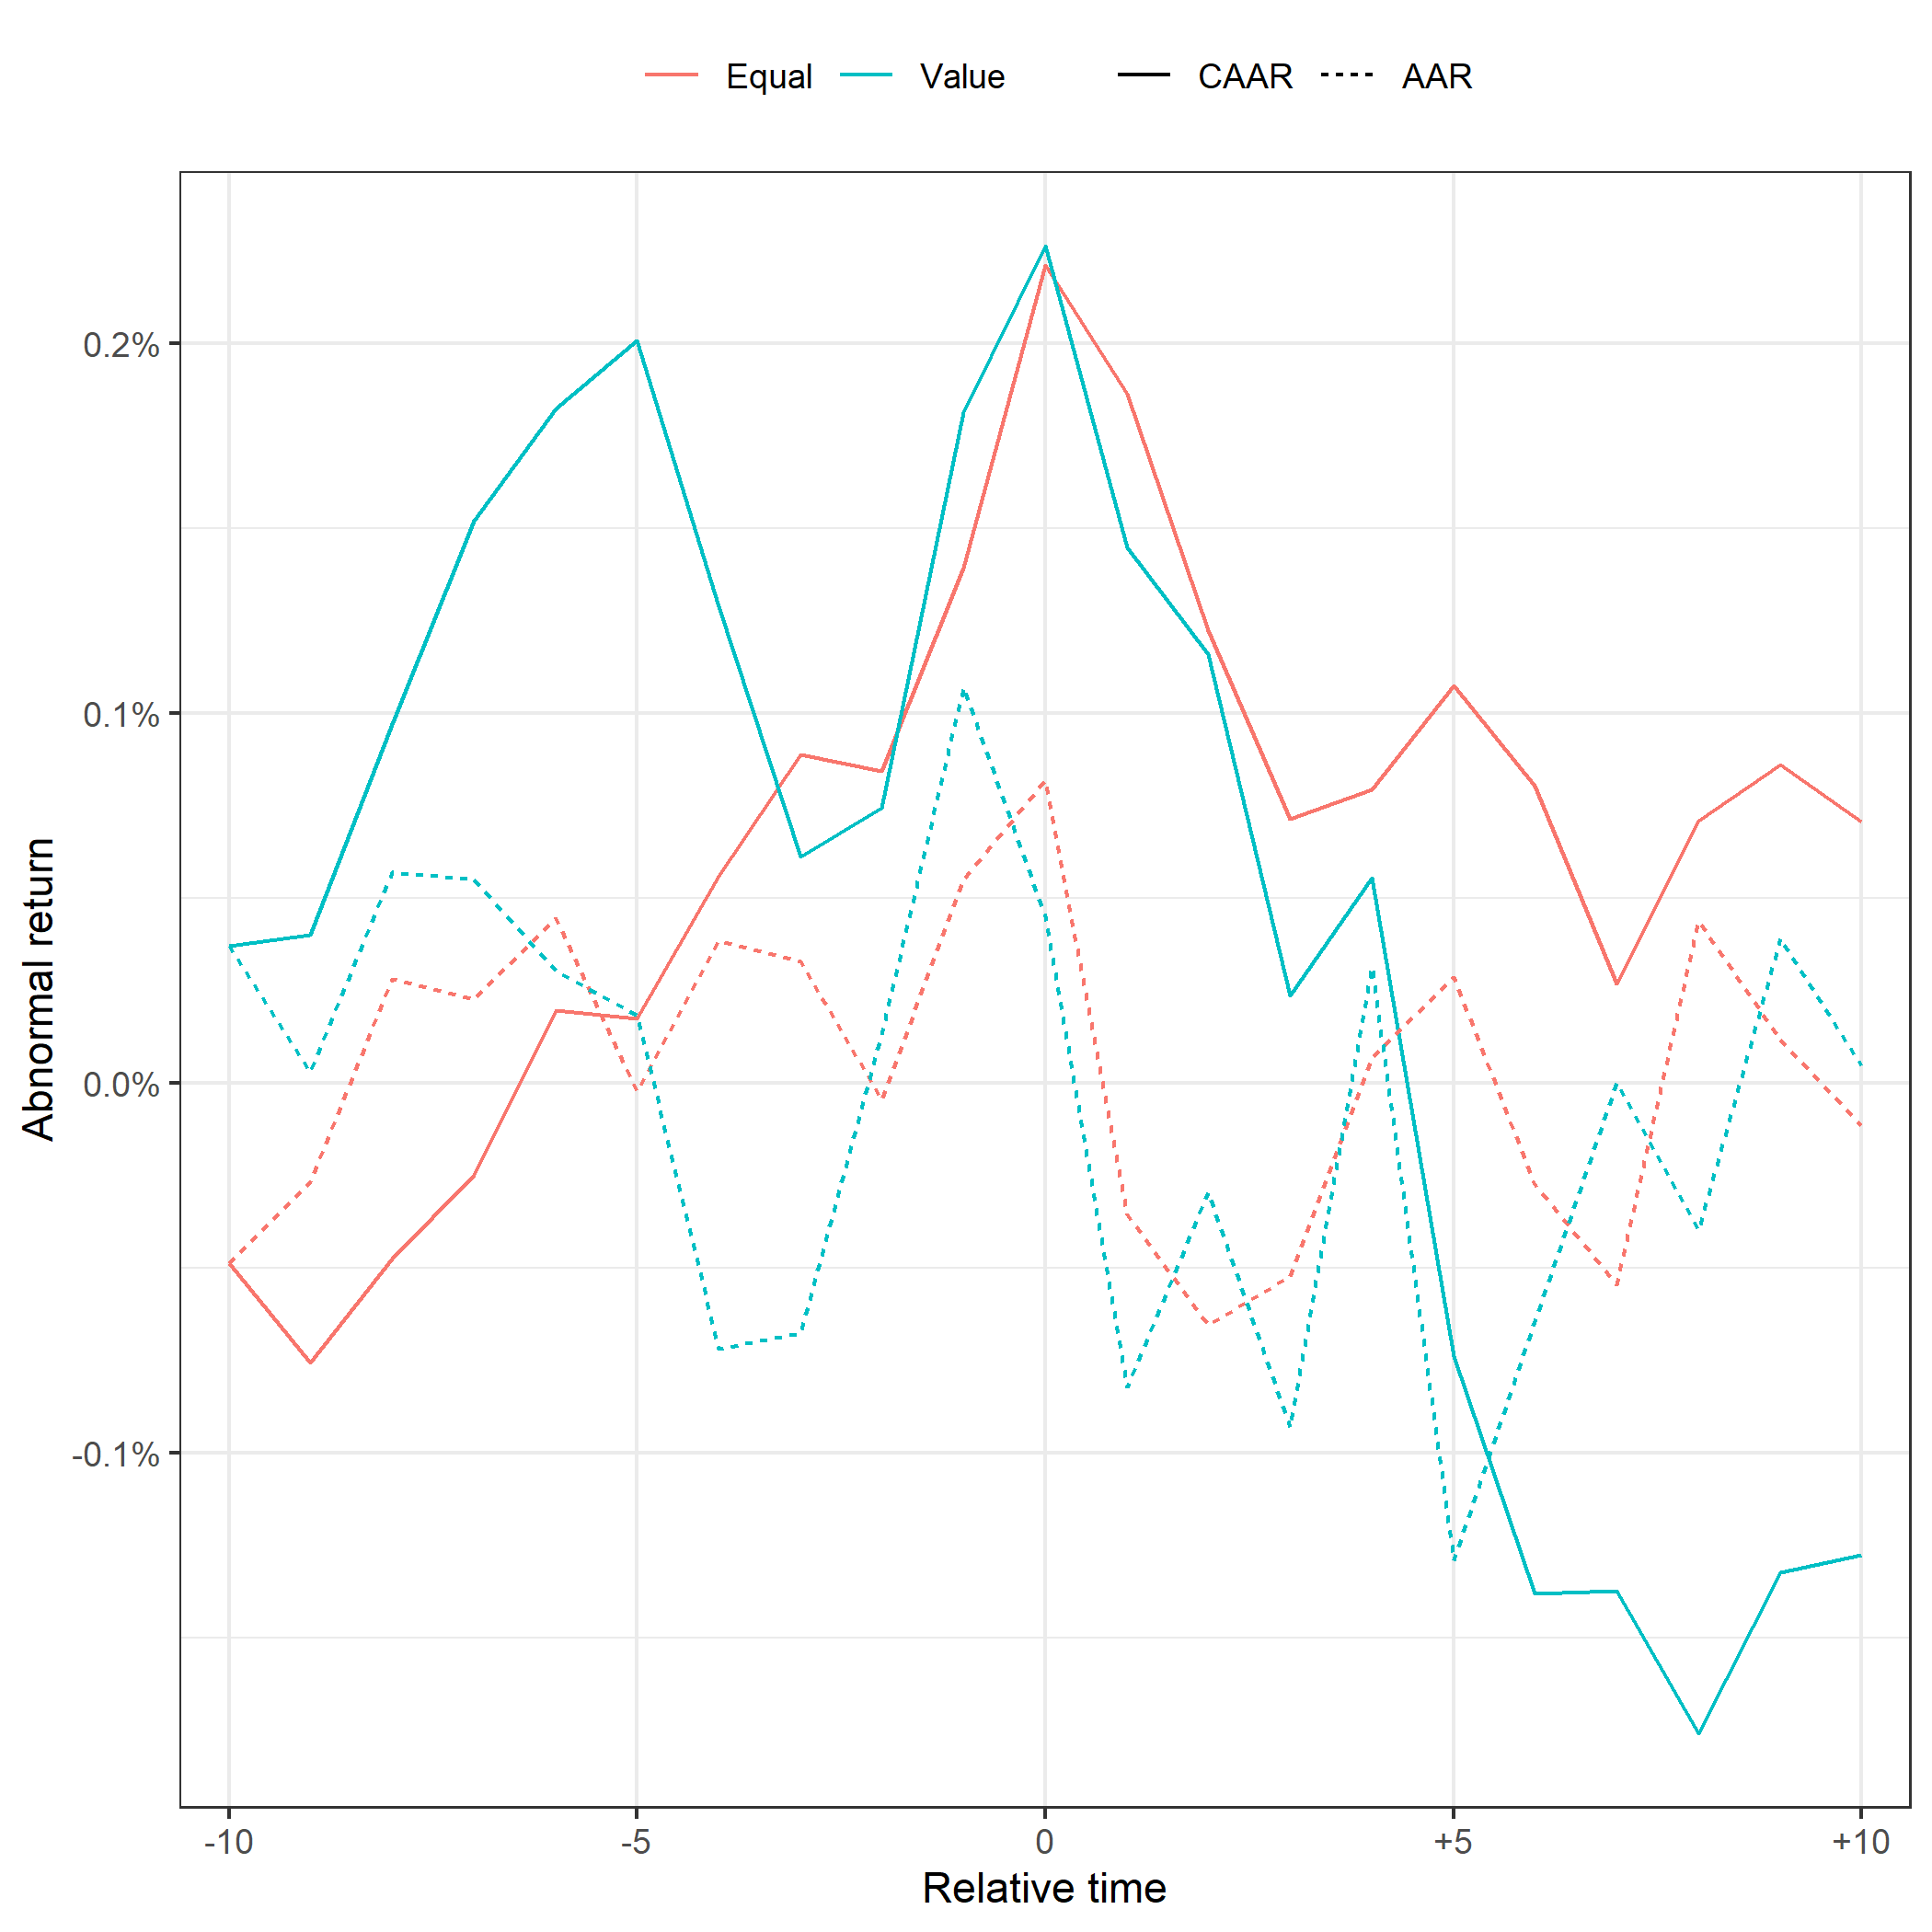
\includegraphics[scale=0.6]{Projekt/1.Figures analysis/ST_positive_sensitivity_weight.png}
     \caption*{\footnotesize The figure illustrates the average abnormal return (AAR) and cumulative AAR (CAAR) around the event date (t = 0) of positive news. The blue lines are returns calculated from an equally weighted portfolio, while the weights of the red lines are based on market capitalization. }
    \label{fig:ST_pos_sensitivity_weights}
\end{figure} 

\subsubsection{Long term}


\setlength{\tabcolsep}{15pt}
\begin{table}[]
\small
\centering
\caption{Fama-French five-factor model alpha from positive news with equal weights} 
\begin{tabular}{ccccccc}
\hline \hline \\ 
 &     &  &    1 SD  &  2 SD  &  3 SD  &  \\ \cline{4-6} 
& & & \multicolumn{3}{c}{ T = 1} & \\ \cline{2-6}
& Alpha (\%)  &  & $ -0.004$  & $-0.000$  & $-0.006$ &  \\
& t-value &  & -1.55 & -0.27  & -1.48 & \\
& & & \multicolumn{3}{c}{ T = 4} & \\ \cline{2-6}
& Alpha (\%)  &  & $ -0.003^{*}$  & $-0.001^{***}$  &  $-005^{**}$ & \\
& t-value & & -1.77  & -0.75 & -227 & \\
& & & \multicolumn{3}{c}{ T = 8} & \\ \cline{2-6}
& Alpha (\%)  &  & $ -0.003^{***}$   & $-0.003^{**}$  & $-0.005^{**}$ &  \\
& t-value &  & -2.98  & -2.45 & 3.51 & \\
&  & & \multicolumn{3}{c}{ T = 12} & \\ \cline{2-6}
& Alpha (\%)  &  & $ -0.004^{***}$  & $-0.003^{**}$  & $-0.003^{**}$ &  \\
& t-value &  & -3.02  & -2.66 & -1.12 & \\
\hline \hline
 \multicolumn{7}{l}{ \footnotesize $^* \; p\; <\; 0.1$, $ ^{**} \; p\; <\; 0.05$, $ ^{***} \; p\; <\; 0.01$  } \\
 \multicolumn{7}{p{11.5cm}}{ \footnotesize Alpha is the WLS-regression intercept (in \%) of the Fama-French 3-factor model, displayed along with the corresponding t-value. N is the average amount of firms included in the portfolio each month, and T is the portfolio holding period. The threshold for event firms to be included in the portfolio is either 1,2 or 3 "SD" (standard deviations) larger than the mean.}  \\ 
\end{tabular}
\label{tab: FF5_pos_equalW}
\end{table}


\setlength{\tabcolsep}{15pt}
\begin{table}[H]
\small
\centering
\caption{FF-5 model alpha from positive news with altered event identification rule } 
\begin{tabular}{ccc}
\hline \hline \\ 
&  2 SD  &  3 SD   \\ \cline{2-3} 
 \multicolumn{2}{c}{ T = 1}  \\ \hline
 Alpha (\%) & 0.04  & -0.37   \\
 t-value & 0.11  & -0.74  \\
 \multicolumn{2}{c}{ T = 4}  \\ \hline
 Alpha (\%)  & 0.03  &  -0.07  \\
 t-value  & 0.13  & -0.23  \\
 \multicolumn{2}{c}{ T = 8}  \\ \hline
 Alpha (\%) & -0.01  & 0.04   \\
 t-value & -0.15 & 0.18  \\
 \multicolumn{2}{c}{ T = 12}  \\ \hline
 Alpha (\%) & 0.13  & 0.23   \\
 t-value & 1.09 & 1.35  \\
 \hline \hline
 \multicolumn{3}{l}{ \footnotesize $^* \; p\; <\; 0.1$, $ ^{**} \; p\; <\; 0.05$, $ ^{***} \; p\; <\; 0.01$  } \\
 \multicolumn{3}{p{5cm}}{ \footnotesize Alpha is the WLS-regression intercept (in \%) of the Fama-French 5-factor model, displayed along with the corresponding t-value. N is the average amount of firms included in the portfolio each month, and T is the portfolio holding period. The threshold for event firms to be included in the portfolio is either 1,2 or 3 standard deviations (SD) larger than the mean.}  \\ 
\end{tabular}
\label{tab: FF5_pos}
\end{table}

\pagebreak



\end{document}